\documentclass[]{iat}
%Diese Beiden Pakete werden nur für das Beispieldokument benötigt und sollten von Ihnen gelöscht werden
\usepackage{listings}
\usepackage{scrhack}
\usepackage{algorithm2e}
\usepackage{placeins}
\usepackage{amsmath}
%Hier können weitere benötigte Pakete Eingebunden werden

%Namen eingeben / Insert Name
\renewcommand{\author}{Dasanayake Mudiyanselage Hasith Thilanka Dasanayake}
%Art der Arbeit / Scope (Project, Thesis...)
\providecommand{\scope}{Projektarbeit}
%Thema der Arbeit / Theme of Thesis
\renewcommand{\subject}{Line Segment Detection}
%Schlagwörter / Keywords
\providecommand{\keywords}{Key_1, Key_2}
%Literaturliste *.bib / Bibliography
\providecommand{\bibfile}{IAT_Beispiel_literature}
%Matrikelnummer / Student ID
\providecommand{\studentID}{6003143}
%Betreuer /& Tutors
\providecommand{\tutora}{Stadler}
%Prüfer / Examiner
\providecommand{\examinera}{Jekyll}


\hypersetup{%
	pdftitle	={\subject -- \author -- \today},
	pdfauthor	={\author},
	pdfsubject	={\subject},
	pdfkeywords ={\keywords}
}

\bibliography{\bibfile} 

\setlength{\footheight}{21pt}

\begin{document}
	\lstset{literate={ä}{{\"a}}1}
%Pfad zu Grafiken:
	\graphicspath{{./project_graphics/}}
% Sprachauswahl /Language Selection (ngerman/english)
	\selectlanguage{english}
\pagenumbering{roman}
\input{iat_title}
%Urherberrechtserklärung / Confirmation of Conformity Comment if not needed, Select correct Language
\input{declaration_conformity}
\pagestyle{iat}
\tableofcontents
\chapter{Introduction}
\pagenumbering{arabic}
\setcounter{page}{1}
\par
This section is under construction. 
\par
\chapter{Methodology}
Line Segment Detection (LSD) is the most common and essential step in computer vision. The major challenges in LSD such as accurate segment selection out of several segments, and the efficient processing of the algorithm, have been extensively investigated.
\par
In this research, Run-Length Encoded (RLE) and annotated images in JSON format were used as the initial data source for the implementation of the Line Segment Detection Algorithm. After RLE data has been decoded to an image, preprocessing and preparation steps were described in section 2.2. Then in section 2.3, the feature extraction step was described. Which is the most important step to detect all the line segments in the image. In the final step, (section 3.4) line segments between two bounding boxes were successfully identified on the stem of each plant. Fig. shows the methodology in a flow chart.
\\
\section{Preprocessing and Preparation}
In this project, an image annotation tool called “Hasty” was used to create a ground-truth dataset. During the annotation, the object classes of the image were defined as “First Section Cutting”, “Redundant Top End” and “Tip Cutting” etc. Finally, the annotated image was encoded to a run-length encoded (RLE) binary mask, which is a compressed representation of a binary image. In this encoding, the binary image is represented by a sequence of pairs (start, length), where each pair represents a consecutive run of 1's in the image. 
\par
In the 1st part of the algorithm, this mask was decoded and created a 2D numpy array. Also, image dimensions, bounding box details, and selected object classes (First Section Cutting, Redundant Top End, Redundant Bottom End, Tip Cutting, Non-Viable Part, Second Section Cutting, Third Section Cutting, Fourth Section Cutting) which are useful for the line segment detection were gathered in this stage.
\par
Usually, sample images contain one or more plants, and in the second part of the algorithm, two Python lists were generated. Typically, in the Hasty Generated JSON file, plant sections are annotated with specific small bounding boxes and saved separately. The exact coordinates of these small bounding boxes were stored in the first Python list (Let’s call “small\_bbox\_list”). Also, large bounding boxes were defined for each plant (with all the section cuttings) in the JSON file and saved separately in the second Python list (Let’s call “large\_bbox\_list”). In addition, a dictionary was created to store the details of each plant section. In this case, the background of the image was saved as "0" and the foreground as "1". As Shown in the  \autoref{fig:fig2} one large bounding box consisted of multiple small bounding boxes. 
\par
\FloatBarrier
\begin{figure}[h]
    
	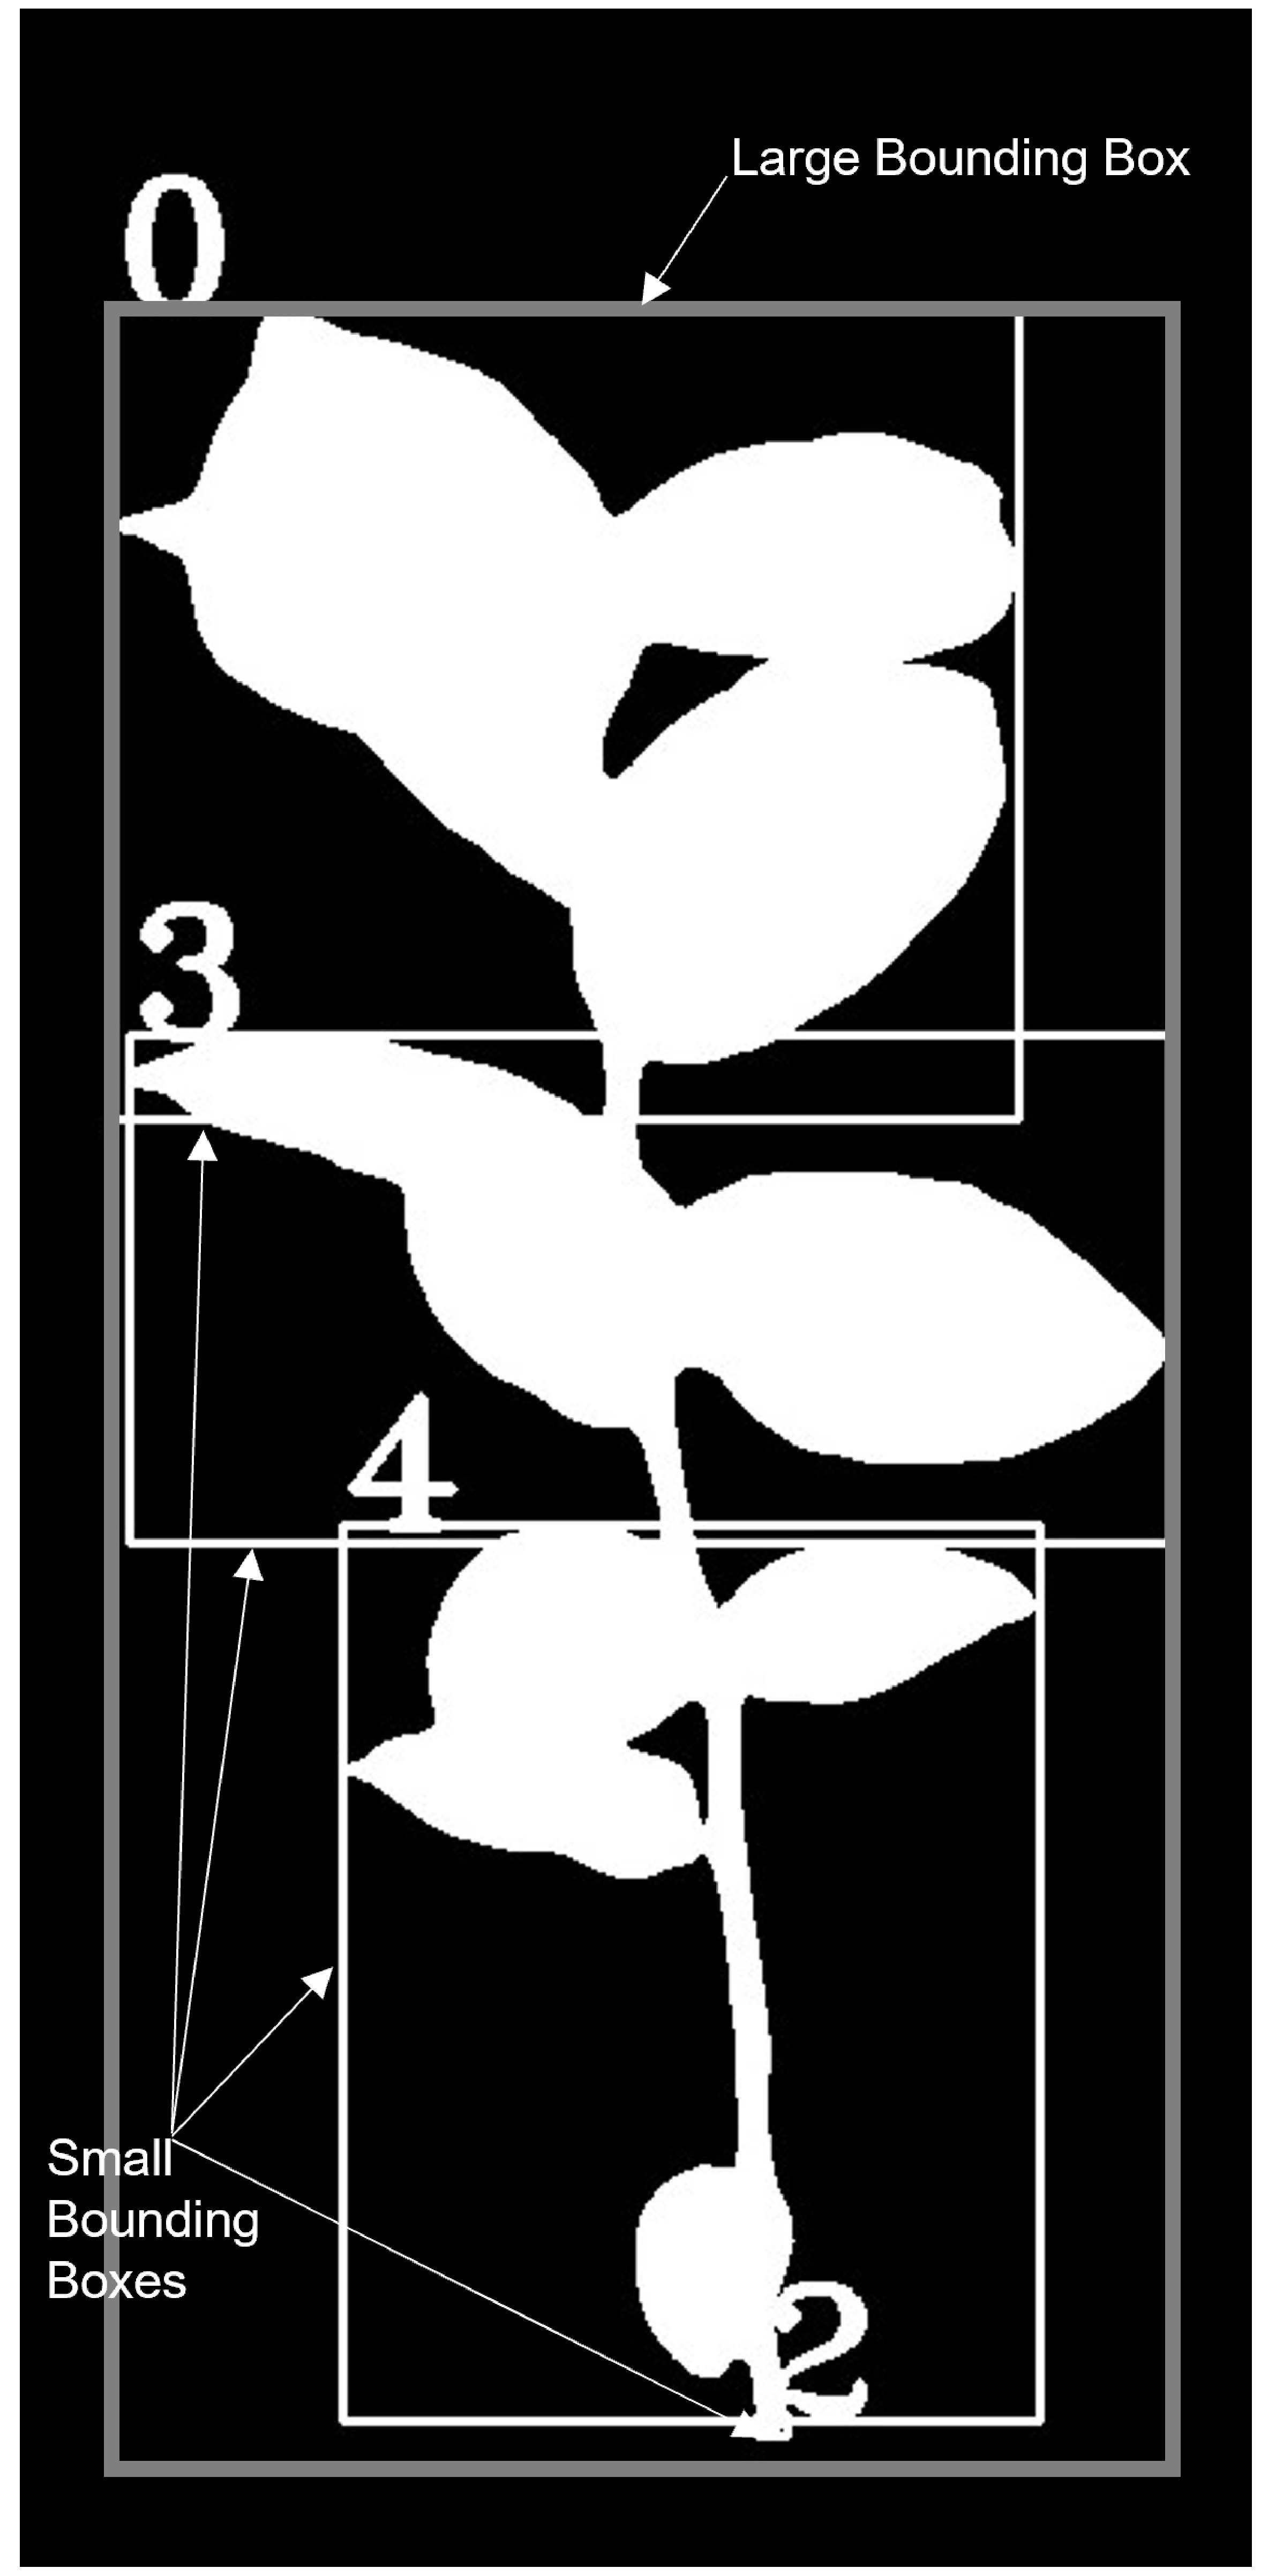
\includegraphics[width=0.4\textwidth]{project_graphics/Fig2.eps}
	\caption{Small and Large Bounding Boxes}
	\label{fig:fig2}
\end{figure}


Then the 3rd part of the algorithm was used to create the list of neighboring sections of the plants. As an example, 1st section, and 2nd section of the plant . This part of the algorithm is more challenging because efficiency of the algorithm mainly depends on this section. In here, OpenCV function: cv2.findContours() was used to detect only the external contours (cv2.RETR\_EXTERNAL) of the sections of the plants and saved them in a list(Let’s call “edge\_only\_list”). Then in order to reduce the memory usage and speed up the process “cv2.CHAIN\_APPROX\_SIMPLE” method was used as the contour approximation method. Initially, both internal (whole solid section of the plant) and external contours were used to find the neighboring sections of the plants. But during the stage of optimizing the algorithm’s efficiency, huge efficiency improvements were achieved while using this outside contour detection method. It was discussed more in the results section.
\par
Also, an additional major improvement in efficiency was achieved through the utilization of parallel processing. By considering the factor of ease of use, two types of parallel processing methods were tested, which were based on multiple threads and multiple processors. The use of multiple processors for parallel processing involves the distribution of the workload across numerous physical or logical processors. Consequently, this particular aspect of the algorithm (the identification of neighboring sections and the identification of complete sections of the plant) was specifically designed to facilitate easy parallel processing. For initial testing, a standard Python library called "multiprocessing" was employed. Regrettably, the processing time exceeded the duration of normal processing. Consequently, an alternative technique based on multiple threads was adopted, utilizing the "concurrent.futures" module in Python.
\par
A thread is a lightweight unit of execution that can run concurrently with other threads, sharing the same memory space. As shown in the following  \autoref{alg:algo1}, \autoref{alg:algo2},  \autoref{alg:algo3} , multi-threading was used. Finally, identical combinations of neighboring sections were eliminated. For instance, combinations such as (1st section cutting, 2nd section cutting) and (2nd section cutting, 1st section cutting) were considered as similar combinations and were consequently removed from the list of neighboring sections.
\par
\FloatBarrier
\clearpage
\begin{algorithm}[htbp]
    \SetAlgoLined
    \caption{Finding Neighboring Sections}
    \label{alg:algo1}
    \SetKwInOut{Input}{Input}
    \SetKwInOut{Output}{Output}

    \Input{small\_bbox\_list, edge\_only\_list}
    \Output{neighboring\_sections\_list, intersected\_area\_list}

    \BlankLine
    Initialize an empty list neighboring\_sections\_list; Initialize an empty list intersected\_area\_list\;

    \BlankLine
    \ForEach{mask\_index in small\_bbox\_list}{
        \ForEach{mask\_index\_checked in edge\_only\_list}{
            \ForEach{ones\_index in edge\_only\_list[mask\_index\_checked]}{
                \If{(\(small\_bbox\_list[mask\_index][0] \leq edge\_only\_list[mask\_index\_checked][ones\_index][1] < small\_bbox\_list[mask\_index][1]\)) \textbf{and} (\(small\_bbox\_list[mask\_index][2] \leq edge\_only\_list[mask\_index\_checked][ones\_index][0] < small\_bbox\_list[mask\_index][3]\))}{
                    \If{mask\_index $\neq$ mask\_index\_checked}{
                        Append [mask\_index, mask\_index\_checked] to neighboring\_sections\_list; Append [(edge\_only\_list[mask\_index\_checked][ones\_index][0], edge\_only\_list[mask\_index\_checked][ones\_index][1]), mask\_index, mask\_index\_checked] to intersected\_area\_list\;
                    }
                }
            }
        }
    }

    \BlankLine
    \Return(neighboring\_sections\_list, intersected\_area\_list)\;
\end{algorithm}

\FloatBarrier

\begin{algorithm}[htbp]
    \SetAlgoLined
    \caption{Finding Small BBoxes Inside Large BBox}
     \label{alg:algo2}
    \SetKwInOut{Input}{Input}
    \SetKwInOut{Output}{Output}

    \Input{large\_bbox\_list, edge\_only\_list}
    \Output{mask\_inside\_large\_bbox\_list}

    \BlankLine
    Initialize an empty list mask\_inside\_large\_bbox\_list\;

    \BlankLine
    \ForEach{lg\_bb\_ind and lg\_bb\_ele in large\_bbox\_list}{
        \ForEach{mask\_index\_2 and mask\_ele\_2 in edge\_only\_list}{
            Initialize ones\_count as 0\;

            \ForEach{co\_with\_ones\_ele2 in mask\_ele\_2}{
                \If{(\(lg\_bb\_ele[0] \leq co\_with\_ones\_ele2[1] < lg\_bb\_ele[1]\)) \textbf{and} (\(lg\_bb\_ele[2] \leq co\_with\_ones\_ele2[0] < lg\_bb\_ele[3]\))}{
                    Increment ones\_count by 1\;
                }
            }

            \If{ones\_count is equal to the length of mask\_ele\_2}{
                Append [lg\_bb\_ind, mask\_index\_2] to mask\_inside\_large\_bbox\_list\;
            }
        }
    }

    \BlankLine
    \Return(mask\_inside\_large\_bbox\_list)\;
\end{algorithm}

\FloatBarrier
\begin{algorithm}[htbp]
    \SetAlgoLined
    \caption{Parallel Processing}
    \label{alg:algo3}
    \SetKwInOut{Input}{Input}
    \SetKwInOut{Output}{Output}

    \Input{small\_bbox\_list, large\_bbox\_list, edge\_only\_list}
    \Output{results}

    \BlankLine
    Create an executor using ThreadPoolExecutor\;

    \BlankLine
    Submit the first for loop as a task\;
    task1 = executor.submit(finding\_neighbors, small\_bbox\_list, edge\_only\_list)\;

    \BlankLine
    Submit the second for loop as a task\;
    task2 = executor.submit(finding\_sections, large\_bbox\_list, edge\_only\_list)\;

    \BlankLine
    Wait for both tasks to complete\;
    results = [task1.result(), task2.result()]\;

    \BlankLine
    Combine the results from both tasks and return them\;
    \Return(results)\;
\end{algorithm}

\section{Feature Extraction}

The feature extraction step is the most important step in this project because the cutting line segment of two neighboring sections is situated on the edge. Therefore, several edge detection methods were tested to get optimum results.
\par
In this project, the most important step is the feature extraction step due to the placement of the cutting line segment of two neighboring sections on the edge. Consequently, several edge detection methods were employed to achieve optimum results.
\par
The initial detection method employed in this study was the Canny Edge Detection method (by using Opencv based algorithm (cv2.Canny)), which theoretically encompasses several steps: Firstly, a Gaussian filter was utilized to smooth the image and reduce noise. Subsequently, the gradients of the image intensity were calculated using the Sobel operator. To thin the edges and retain only the maximum values, non-maximum suppression was applied. Pixels were classified as strong, weak, or non-edges through the utilization of double thresholding. Finally, weak edges that are connected to strong edges are retained as actual edges using a process called edge tracking by hysteresis. 
\par
During the analysis of the results, certain line segments were not identified. Consequently, an alternative method was employed to identify these missing line segments. In this study, the Sobel operator (cv2.Sobel) was applied in both the x and y directions, and the resulting outcomes were merged. Usually, the Sobel Operator is utilized to compute the gradient magnitude and direction of an image, facilitating the detection of regions exhibiting substantial changes in intensity. 
\par
Moreover, the identification of edges was performed using the Laplacian of Gaussian (LoG) method. The regions of rapid intensity changes were highlighted by applying a combination of the Laplacian operator (cv2.Laplacian) and Gaussian smoothing (cv2.GaussianBlur) with a kernel size of 3x3. Subsequently, the results obtained from two neighboring plant sections were subjected to an AND operator. The output was then considered further. Finally, various types of line segments were revealed. The stem of the plants exhibited the majority of the line segments, although some irrelevant lines were observed in the area where leaves intersected with each other and with the stems, among others (see \autoref{fig:fig3}).
\FloatBarrier
\clearpage
\begin{figure}[h]
    
	
\includegraphics[width=\textwidth]{project_graphics/Fig3.eps}
	\caption{Intersection of Two Leaves and Leaf and Stem in Two Neighboring Sections}
	\label{fig:fig3}
\end{figure}

\section{Detection of Exact Cutting Line Segment (Classification)}

The most challenging area of the algorithm is encountered when not all line segments are situated on the stem of the plant. Therefore, the detection of the exact line segment was performed in three steps based on the results of the feature extraction stage. Initially, a combination of nearest sections with single line segments was considered. Subsequently, combinations of nearest sections were identified with multiple line segments, which were further classified into two main categories. These line segments arise primarily from the intersection of two leaves or the intersection of a portion of the leaves and stems. The first classification (second step) was conducted based on the size of the line segments. Data analysis revealed that the majority of the samples exhibited a noticeable difference in size, although some samples exhibited line segments that were nearly similar in size. For this type of sample, the second classification (third step) was employed using the distance of the line segments to the stem.
\par
The first step was easily achieved by utilizing the clustering of the adjacent foreground pixels, as only a single line segment needed to be detected. A threshold value was defined to categorize the cluster of adjacent pixels with non-adjacent pixel clusters. The resulting values were stored in a list called "clustering\_list". (Here, nothing was stored in the "clustering\_list" because all the pixels were adjacent).  Throughout the first step, only one cluster of adjacent pixels (one line segment) was consistently detected. Subsequently, all the pixel coordinates were saved in another list called "cluster\_coor\_list", which served as the final output (detected line segment) of the algorithm.
\par
The second step is executed if the length of the clustering list is found to be non-zero which means multiple line segments are detected. Here, the "cv2.findContours" method was once again employed to detect all available common line segments in two neighboring plant sections. The size of each line segment was measured using "cv2.arcLength()" to identify the range of sizes typically observed on the stem as the cutting line. Based on this range, the correct line segment was detected. As before, the pixel coordinates were saved in the "cluster\_coor\_list".
\par
The third step is pursued only if the size of the line segment falls outside the range or if there are line segments with similar lengths. In this scenario, several methods were attempted to identify the stem of the plant, with the primary concept being to measure the distance from a point in the stem to the nearest line segment.
\par
Initially, a Python library called "PlantCV," designed for image analysis in the field of plant research and based on OpenCV, was utilized to detect the stem. The "plantcv.morphology.skeletonize()" function was applied to obtain the skeletonized image, extracting the skeleton while preserving the plant structure's connectivity. However, a major challenge arose when applying skeletonization to the binary masks representing the plant sections due to the indistinguishable boundary between leaves and stems. Consequently, the algorithm occasionally misidentified leaves as stems and skeletonized them as well. Ultimately, the desired classification of stems and leaves as separate entities was not achieved.
\par
For the same purpose, the next approach involved segmenting the edge of the stem into multiple line segments, as depicted in the figure. The "cv2.createLineSegmentDetector" function was employed, and the result was saved as "LSD\_img". Based on the outcomes, parallel or nearly parallel line segments were observed on either side of the stem. If two or more parallel line segments were sufficiently thickened, the possibility of creating a single line or solid object arose. This technique was utilized to detect stems separately. Consequently, these line segments were dilated using the "cv2.dilate" function with a 7x7 kernel (numpy.ones((7, 7), dtype=np.uint8)) and two iterations. To remove unwanted parts, an erosion operation was applied using the OpenCV erosion function with the same configurations as the dilation function. The difference between the result ("dilated\_eroded\_img") and "LSD\_img" was saved as "subtracted\_img" and subjected to a median blur operation with a kernel size of 7 to reduce noise and outliers.
\par
The resulting image ("subtracted\_img") consisted of disconnected parts of the stem due to improper boundaries where the leaves join. Therefore, another morphological dilation operation was performed to connect those areas as much as possible. Subsequently, the closed and largest contour was assumed to represent the stem, while other small, closed contours were disregarded. The Euclidean distance from that contour to the line segments was calculated, and the line segment with the shortest distance was considered the correct cutting line segment. Finally, the pixel coordinates of that line segment were saved in the "cluster\_coor\_list".
\par
\chapter{Results and Analysis}

In this section, the results of the algorithm for detecting accurate cutting line segments are presented under several subtopics. A JSON file was used, containing a total of 316 images along with varying numbers of plants captured in each image. As an example, in some images, 21 section cuttings were available, while in others, only one or two were available. 
\par
In subtopic 3.1, a selected sample image was considered, and it served as an illustrative example, displaying all the algorithm steps employed. In subtopic 3.2, the accuracy and precision of the algorithm had been evaluated. Furthermore, the efficiency of the algorithm had been considered a critical factor to measure the quality of algorithm. This aspect has been thoroughly described in subtopic 3.3
\par

\section{Visualization of the Algorithm Steps}

As shown in the \autoref{fig:fig4} , all the steps of the algorithm were visualized with the help of an illustrative example(stn2\_pkg004\_0\_1077\_rep). In the feature extraction stage, of the \autoref{fig:fig4} detected line segments were circled in yellow. The details of the  Classification stage were summarized in the \autoref{tab:tab1}. For the index [0, 1], coordinates were received as (887, 1076), (888, 1076), (889, 1077), (890, 1077), (892, 1079), (893, 1079), (892, 1078), (891, 1078), (890, 1077), (889, 1077), (888, 1076). Then for the index [1,2], coordinates were received as (935, 787), (936, 787), (937, 788), (936, 787). 

\par
\FloatBarrier
\clearpage
\begin{figure}[h]
    
	\includegraphics[width=\textwidth]{project_graphics/Fig4.eps}
	\caption{Visualization of Algorithm Steps}
	\label{fig:fig4}
\end{figure}

\FloatBarrier
\begin{table}[h]
\begin{tabular}{crl}
\hline
Neighboring Sections & Index & Classification\\\hline
1st Section and Redundent Botton End & [0, 1] & Using Size \\
1st Section and Raw Cutting & [1, 2] & Using Size \\\hline
\end{tabular}
\caption{Line Segment Coordinates}
\label{tab:tab1}
\end{table}
\section{Evaluation of Algorithm’s Performance }

As mentioned in the introduction, evaluation of this algorithm's performance was done by using 316 samples. Through the analysis of various evaluation metrics and the visualization of results, insights can be gained into how well positive and negative instances are accurately identified by the algorithm. In this project a fundamental tool for summarizing classification results called confusion matrix was used. Moreover, the calculation and interpretation of key evaluation metrics such as accuracy, precision and the F1 score was examined. Furthermore, the Receiver Operating Characteristic (ROC) curve and its significance in assessing the algorithm's performance in terms of Recall and false positive rates was investigated. 
\par
The confusion matrix is a tabular representation of the performance of the algorithm by the counts of true positive (TP), true negative (TN), false positive (FP), and false negative (FN) instances. Then it was used as the basis or the foundation of finding other evaluation metrics. 
\par
As shown in the , the actual classes of “correct line segment available and correct line segment not available” are represented by the columns, while it’s detected(predicted) or not detected are represented by the rows. The number of instances falling into each category is correspondingly indicated by the values in the cells. 
\par
\FloatBarrier
\begin{figure}[h]
    
	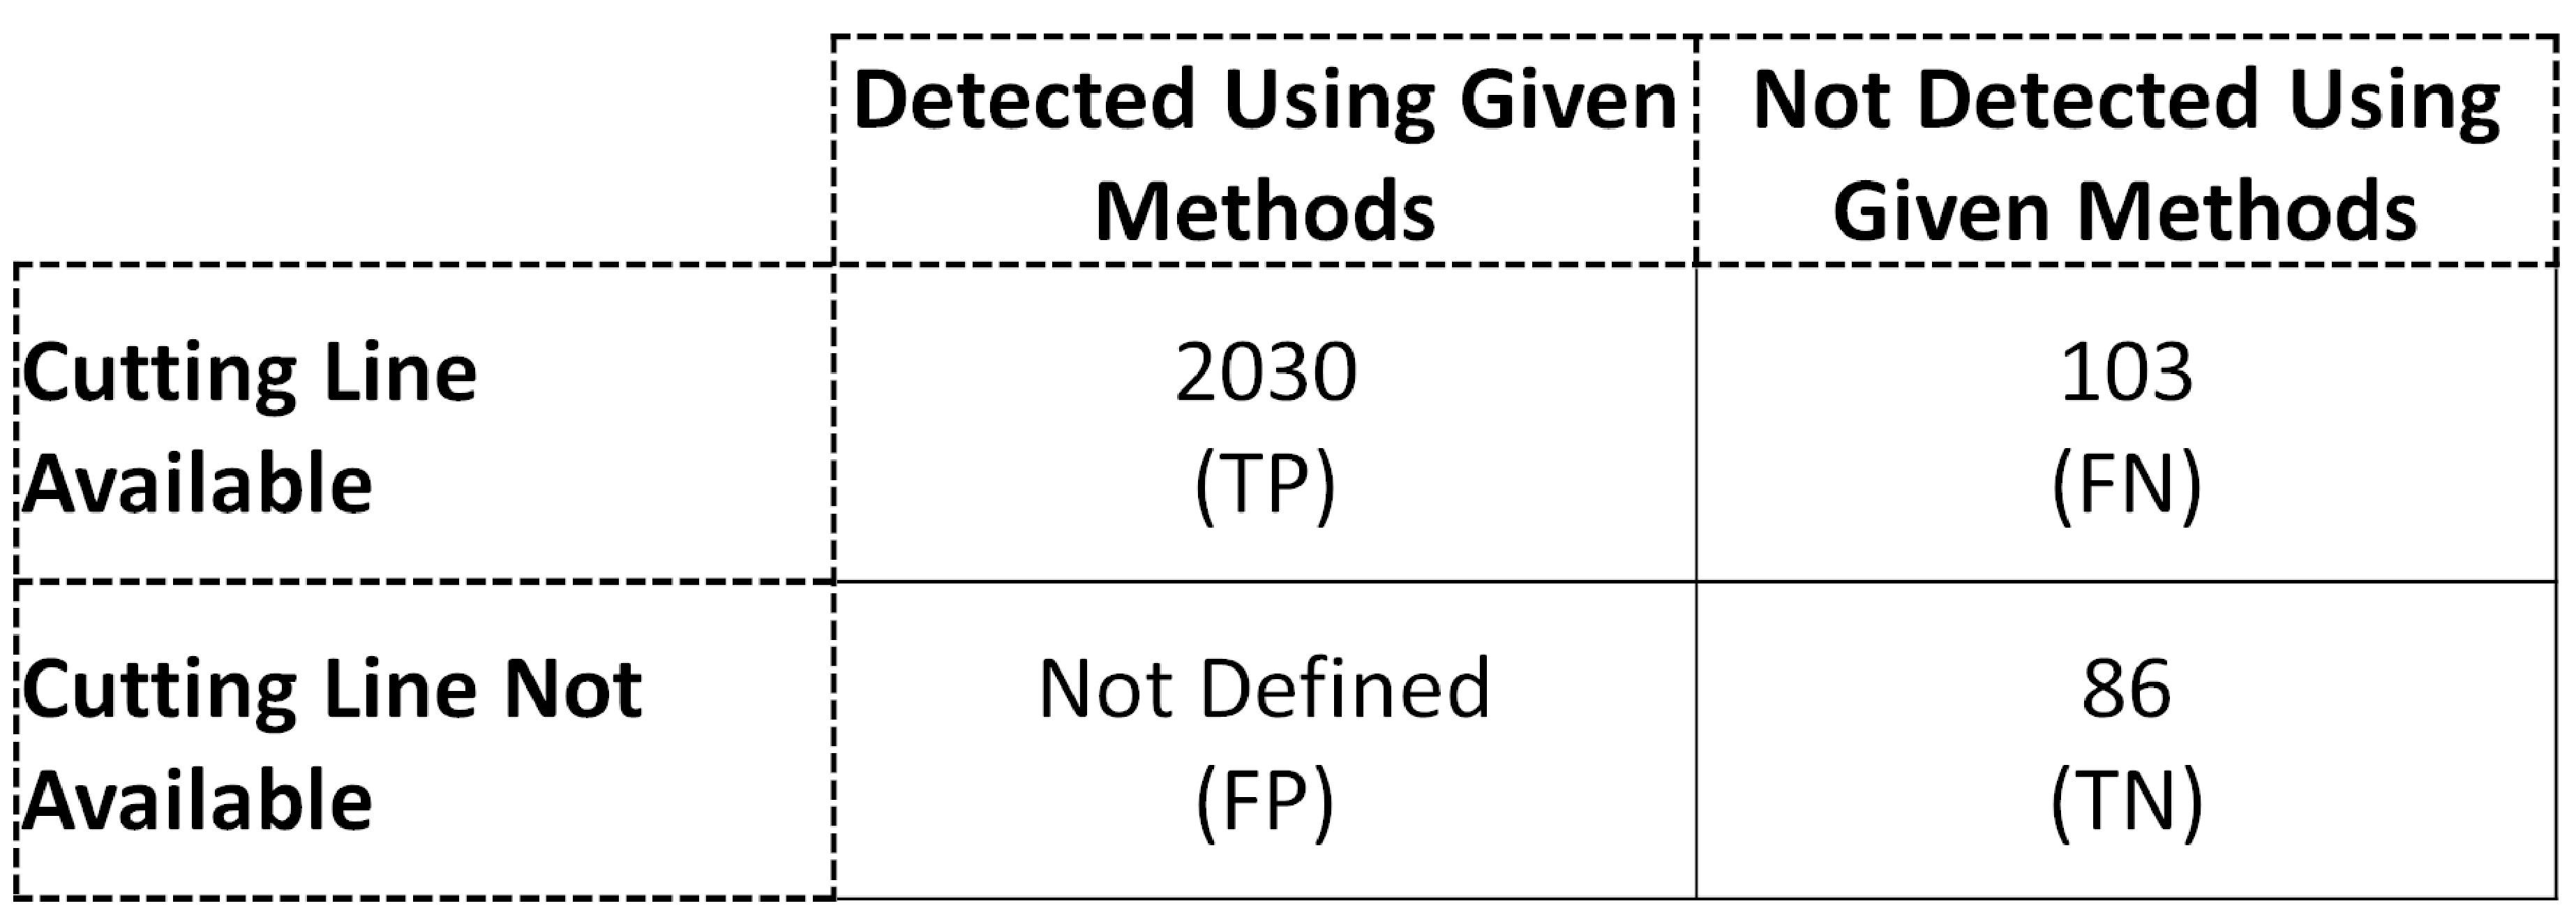
\includegraphics[width=0.5\textwidth]{project_graphics/Fig5.eps}
	\caption{Confusion Matrix}
	\label{fig:fig5}
\end{figure}

The evaluation metrics were computed using the values derived from the confusion matrix. These metrics provide a comprehensive assessment of the algorithm's performance. 
\par
The following formula was used to calculate the accuracy, which measures the overall correctness of the algorithm's predictions.
\FloatBarrier
\begin{align}
Accuracy &=\frac{(TP+TN)}{(TP+TN+FP+FN)}
\end{align}
Initially, the accuracy of the algorithm was calculated with only the 1st step and 3rd detection step of the algorithm (see subtopic 2.4). The accuracy was detected as 0.8912(89.12\%). As shown in the \autoref{fig:fig6} after implementing all three detection steps (see subtopic 2.4) to the algorithm, the accuracy of all the samples was plotted, and the average accuracy was taken as 0.9616 (96.16\%). Therefore, an improvement of 0.0704(7.04\%) was achieved by expanding the detection step. 
\FloatBarrier
\begin{figure}[h]
    
	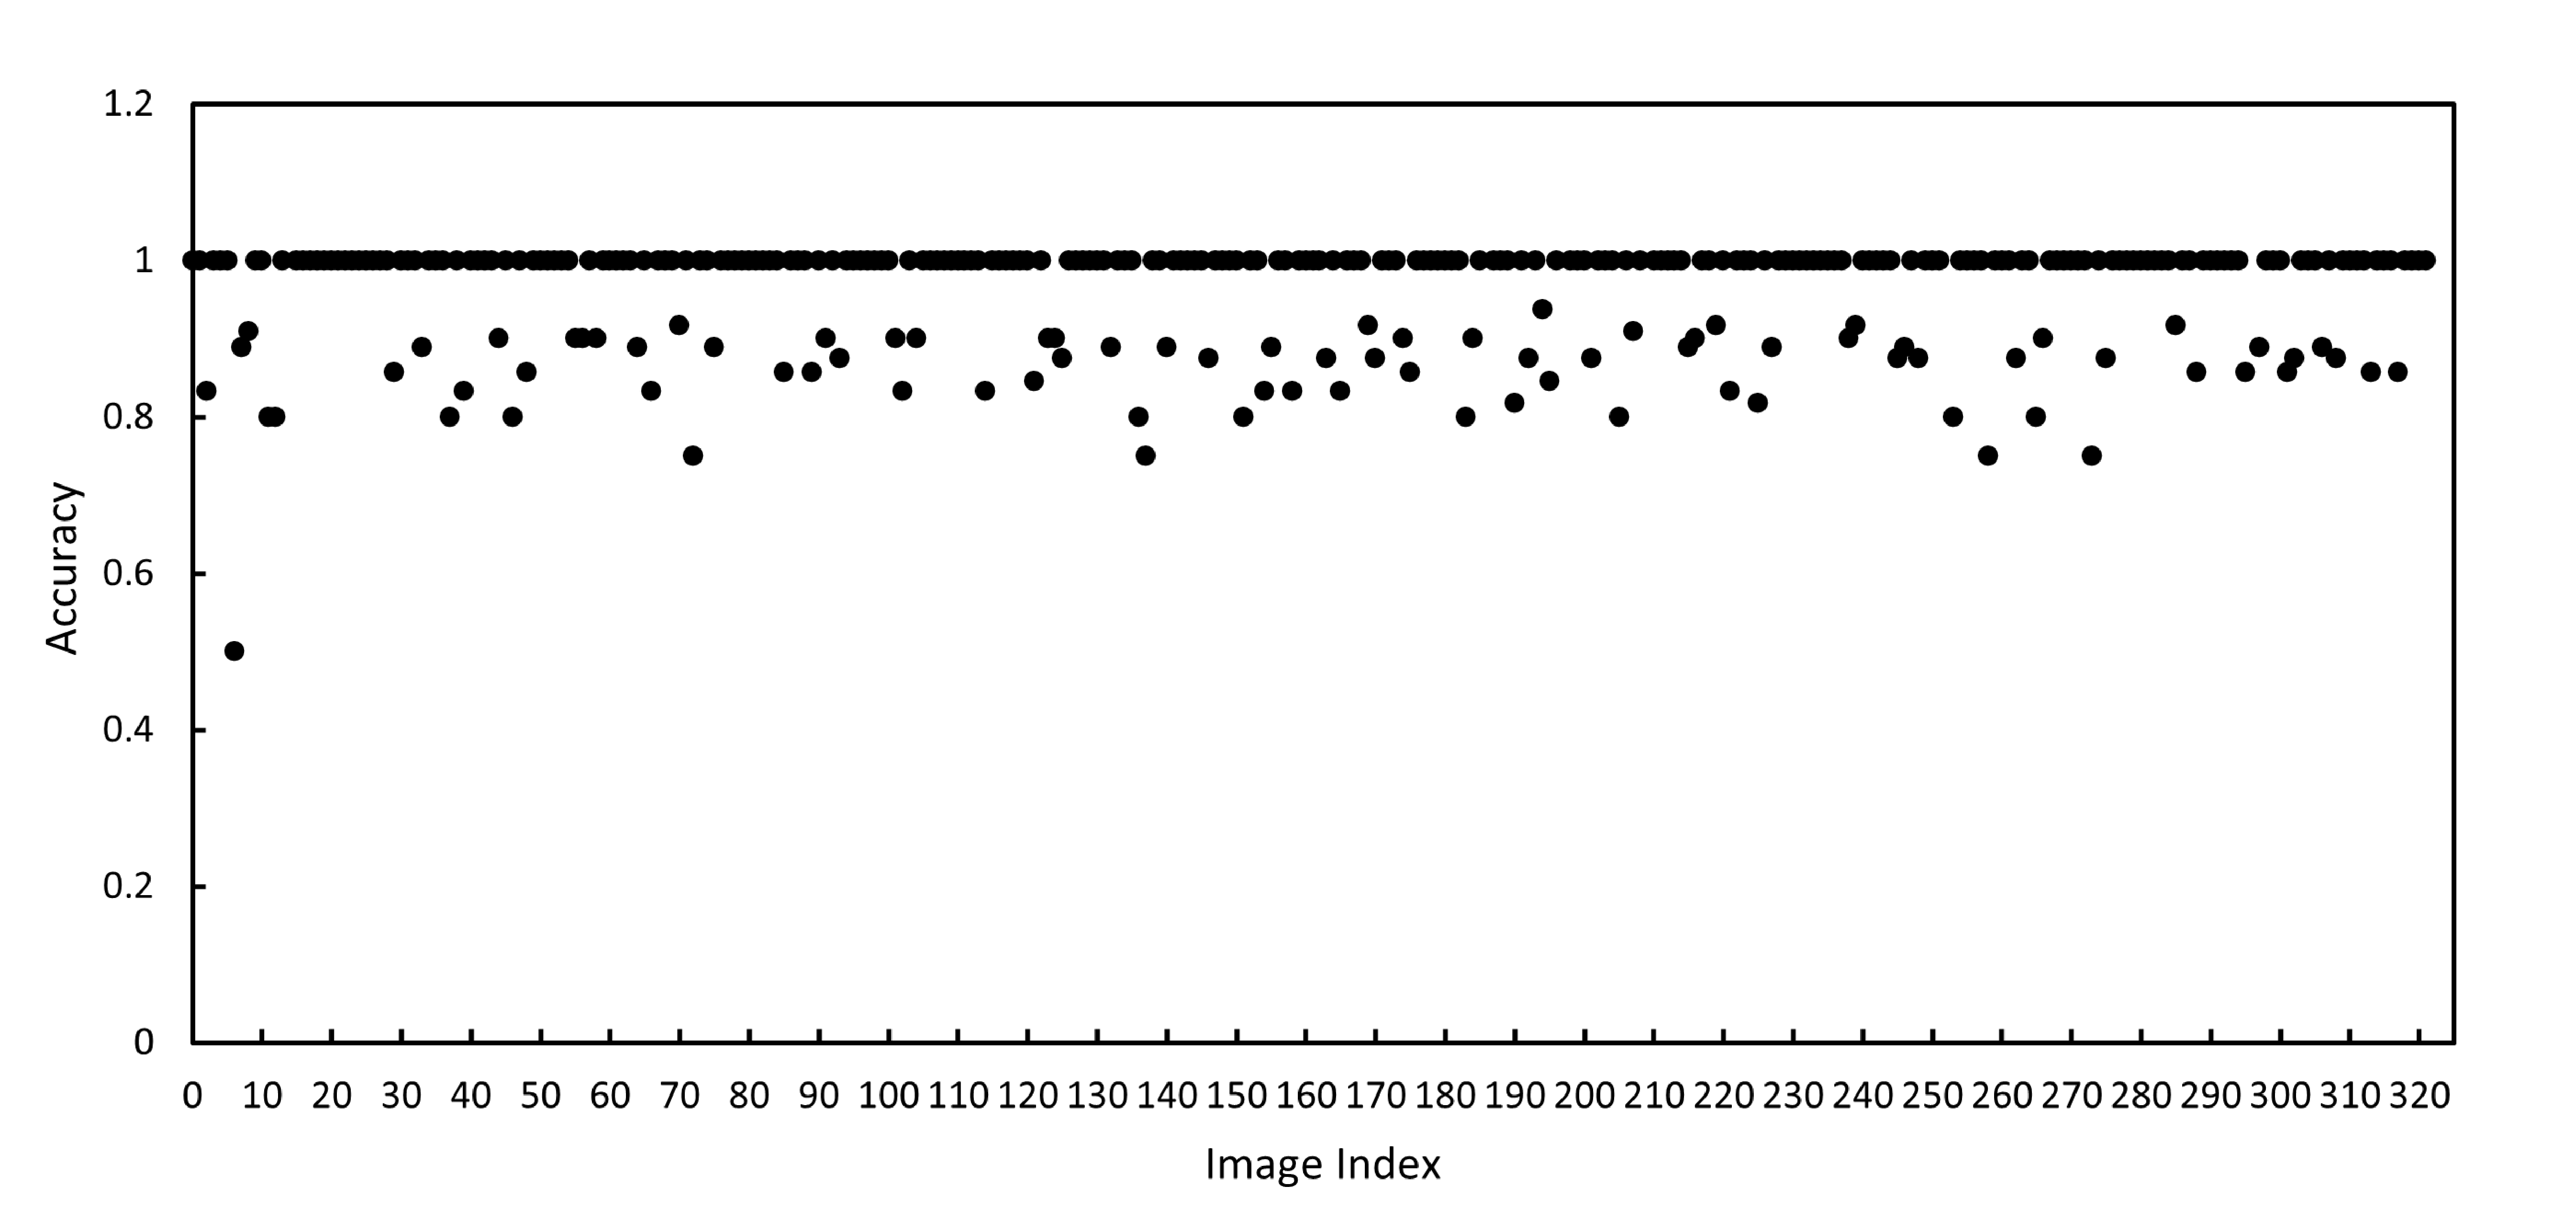
\includegraphics[width=\textwidth]{project_graphics/Fig6.eps}
	\caption{Accuracy vs Image Index Graph}
	\label{fig:fig6}
\end{figure}
\par
This level of accuracy metric indicates a high level of overall correctness in the predictions made by the classification algorithm. Also, the algorithm demonstrates its effectiveness in distinguishing between positive and negative instances (detection and non-detection).
\par
However, a comprehensive analysis of other evaluation metrics is necessary to gain a proper understanding of the algorithm's performance, as well as its strengths and limitations. Therefore, precision and the F1 score were further calculated.
\par
The precision metric evaluates the algorithm's ability to avoid false positive predictions by measuring the proportion of correct positive predictions out of all instances predicted as positive. The following formula represented the precision in terms of the confusion matrix.
\FloatBarrier
\begin{align}
Precision &=\frac{TP}{(TP+FP)}
\end{align}
\FloatBarrier
\begin{figure}[h]
    
	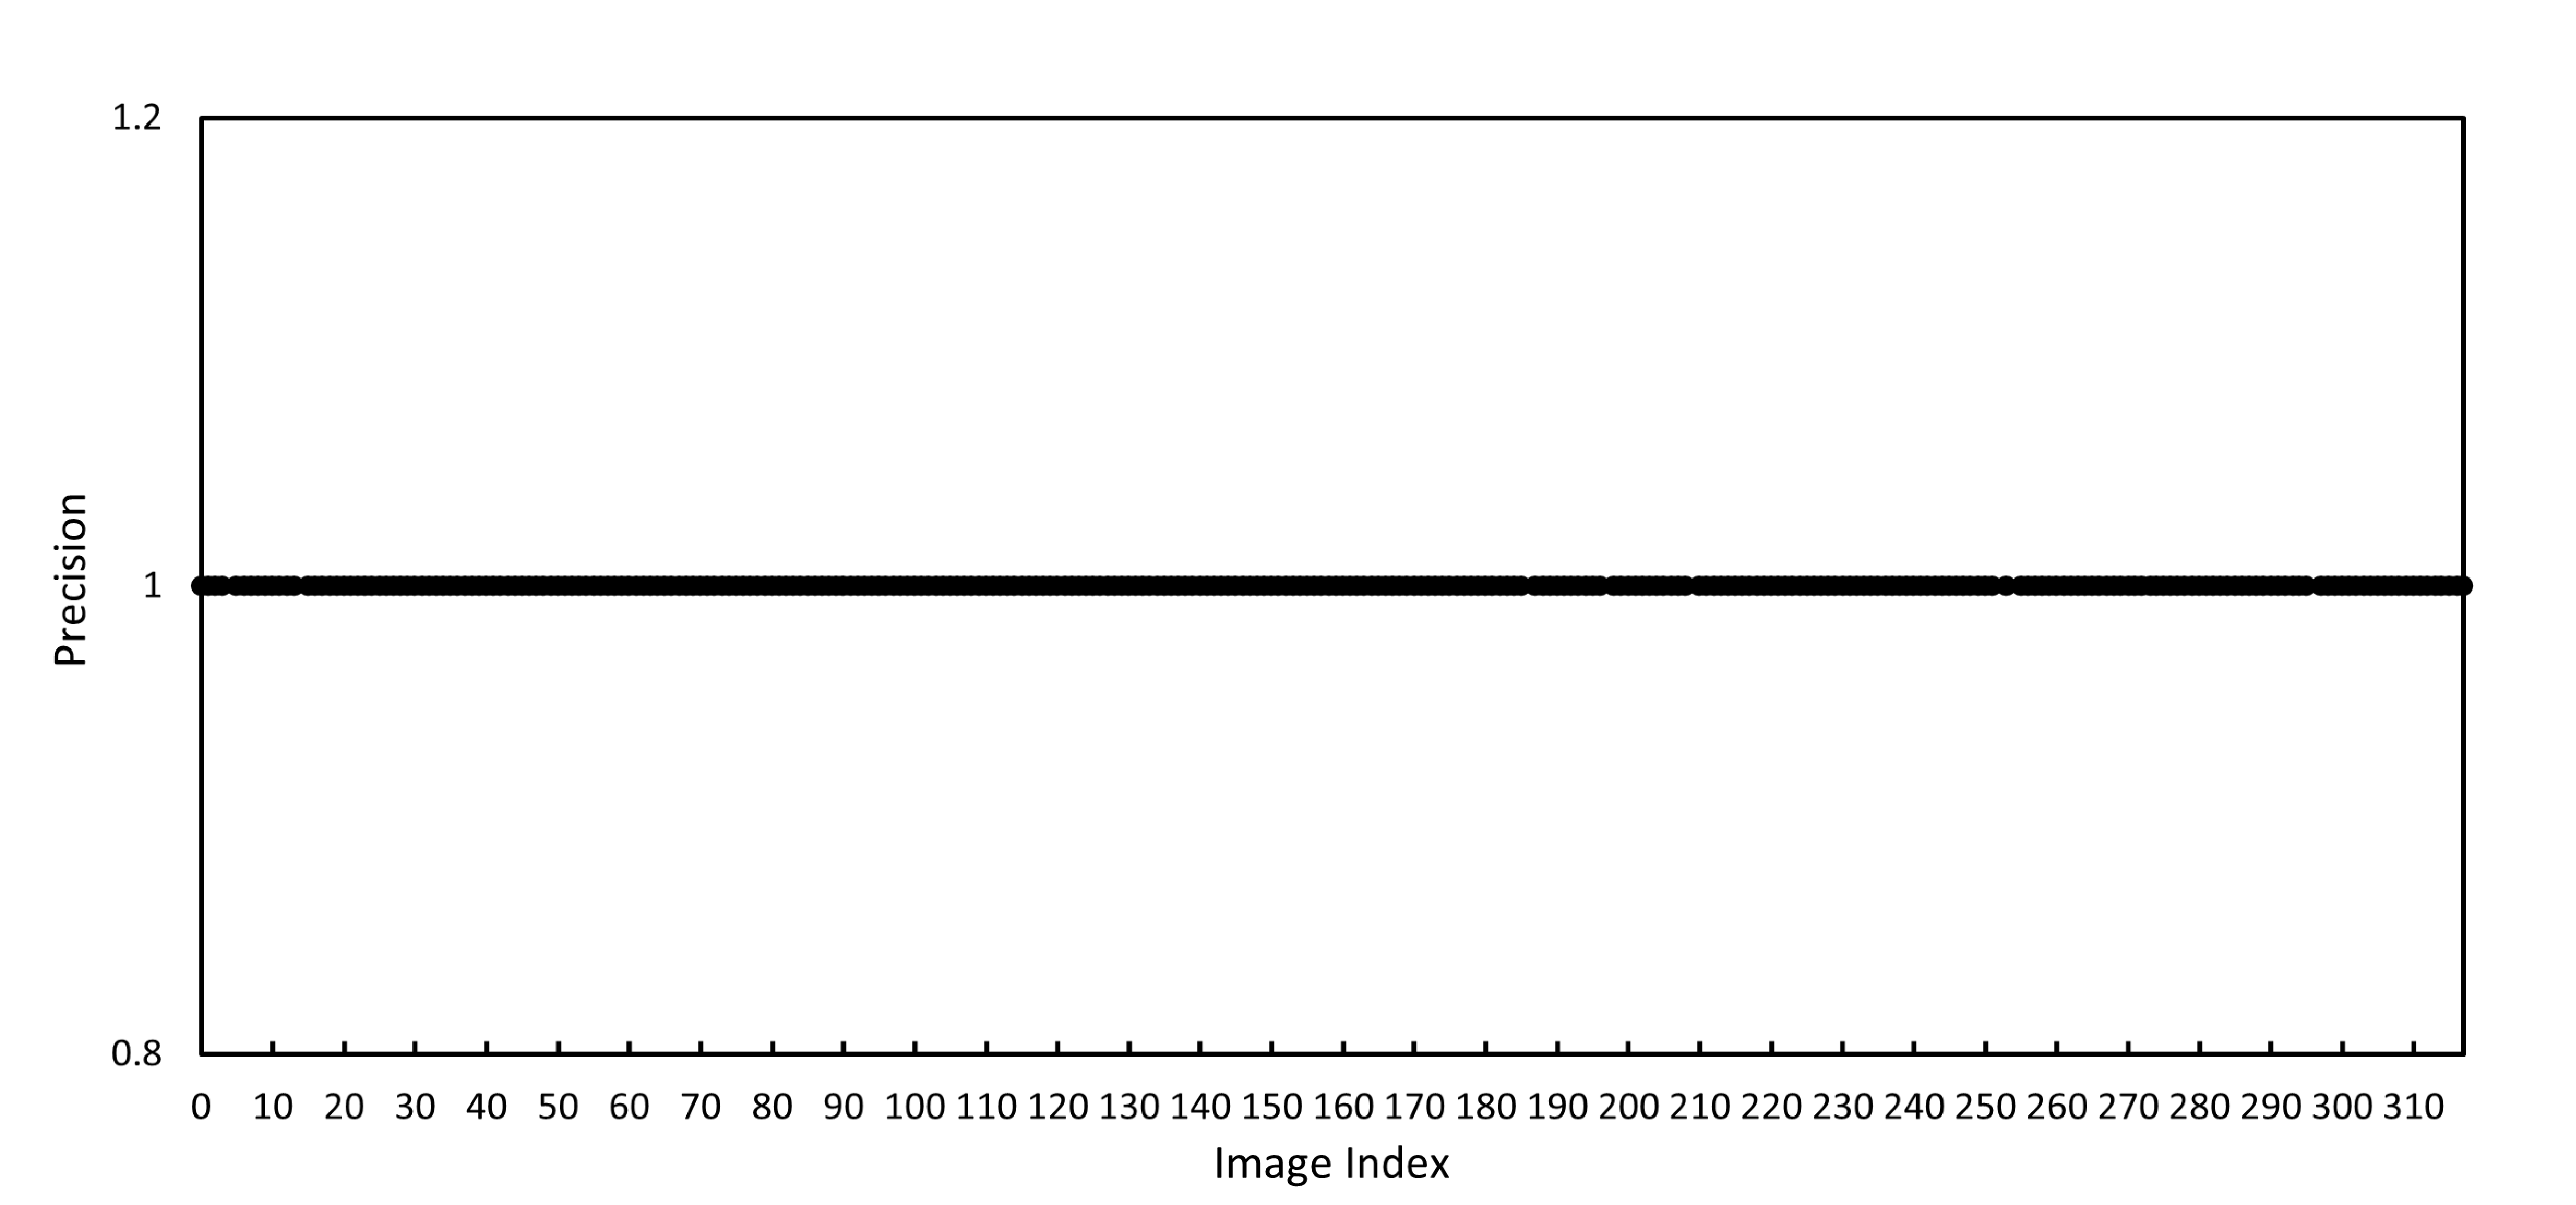
\includegraphics[width=\textwidth]{project_graphics/Fig7.eps}
	\caption{Precision vs Image Index Graph}
	\label{fig:fig7}
\end{figure}
\par
As shown in the \autoref{fig:fig7}. after implementing all three detection steps (see subtopic 2.4) to the algorithm, the precision of all the samples was plotted and the average precision was taken as 0.9608 (96.08\%). As a result, the occurrence of false positives was minimized and making it reliable in distinguishing positive instances from negative ones.
\par
The F1 score, which is determined using the equation provided, represents a balanced measure of the algorithm's performance as it combines both precision and recall in a harmonic mean. These two metrics offer an overall assessment of the algorithm's ability to correctly identify positive instances while minimizing false positives and false negatives.
\par
\FloatBarrier
\begin{align}
F1\_score &=\frac{2*(Precision*Recall)}{(Precision+Recall)}
\end{align}

The average F1 score was achieved as (0.9785) 97.85\%, which indicates that the algorithm achieves a high balance between precision and recall. Here, recall (TP / (TP + FN)) for all the samples was calculated as one because there were zero instances in which the correct line segment was not detected. (Unless it was not passed from the feature extraction section to the classification section of the algorithm.)
\par
As depicted in the \autoref{fig:fig8} higher F1 score was shown. It shows that the algorithm is performing well in terms of correctly identifying positive instances (exhibiting high precision) and minimizing false negatives (demonstrating high recall). 
\par
\FloatBarrier
\begin{figure}[h]
    
	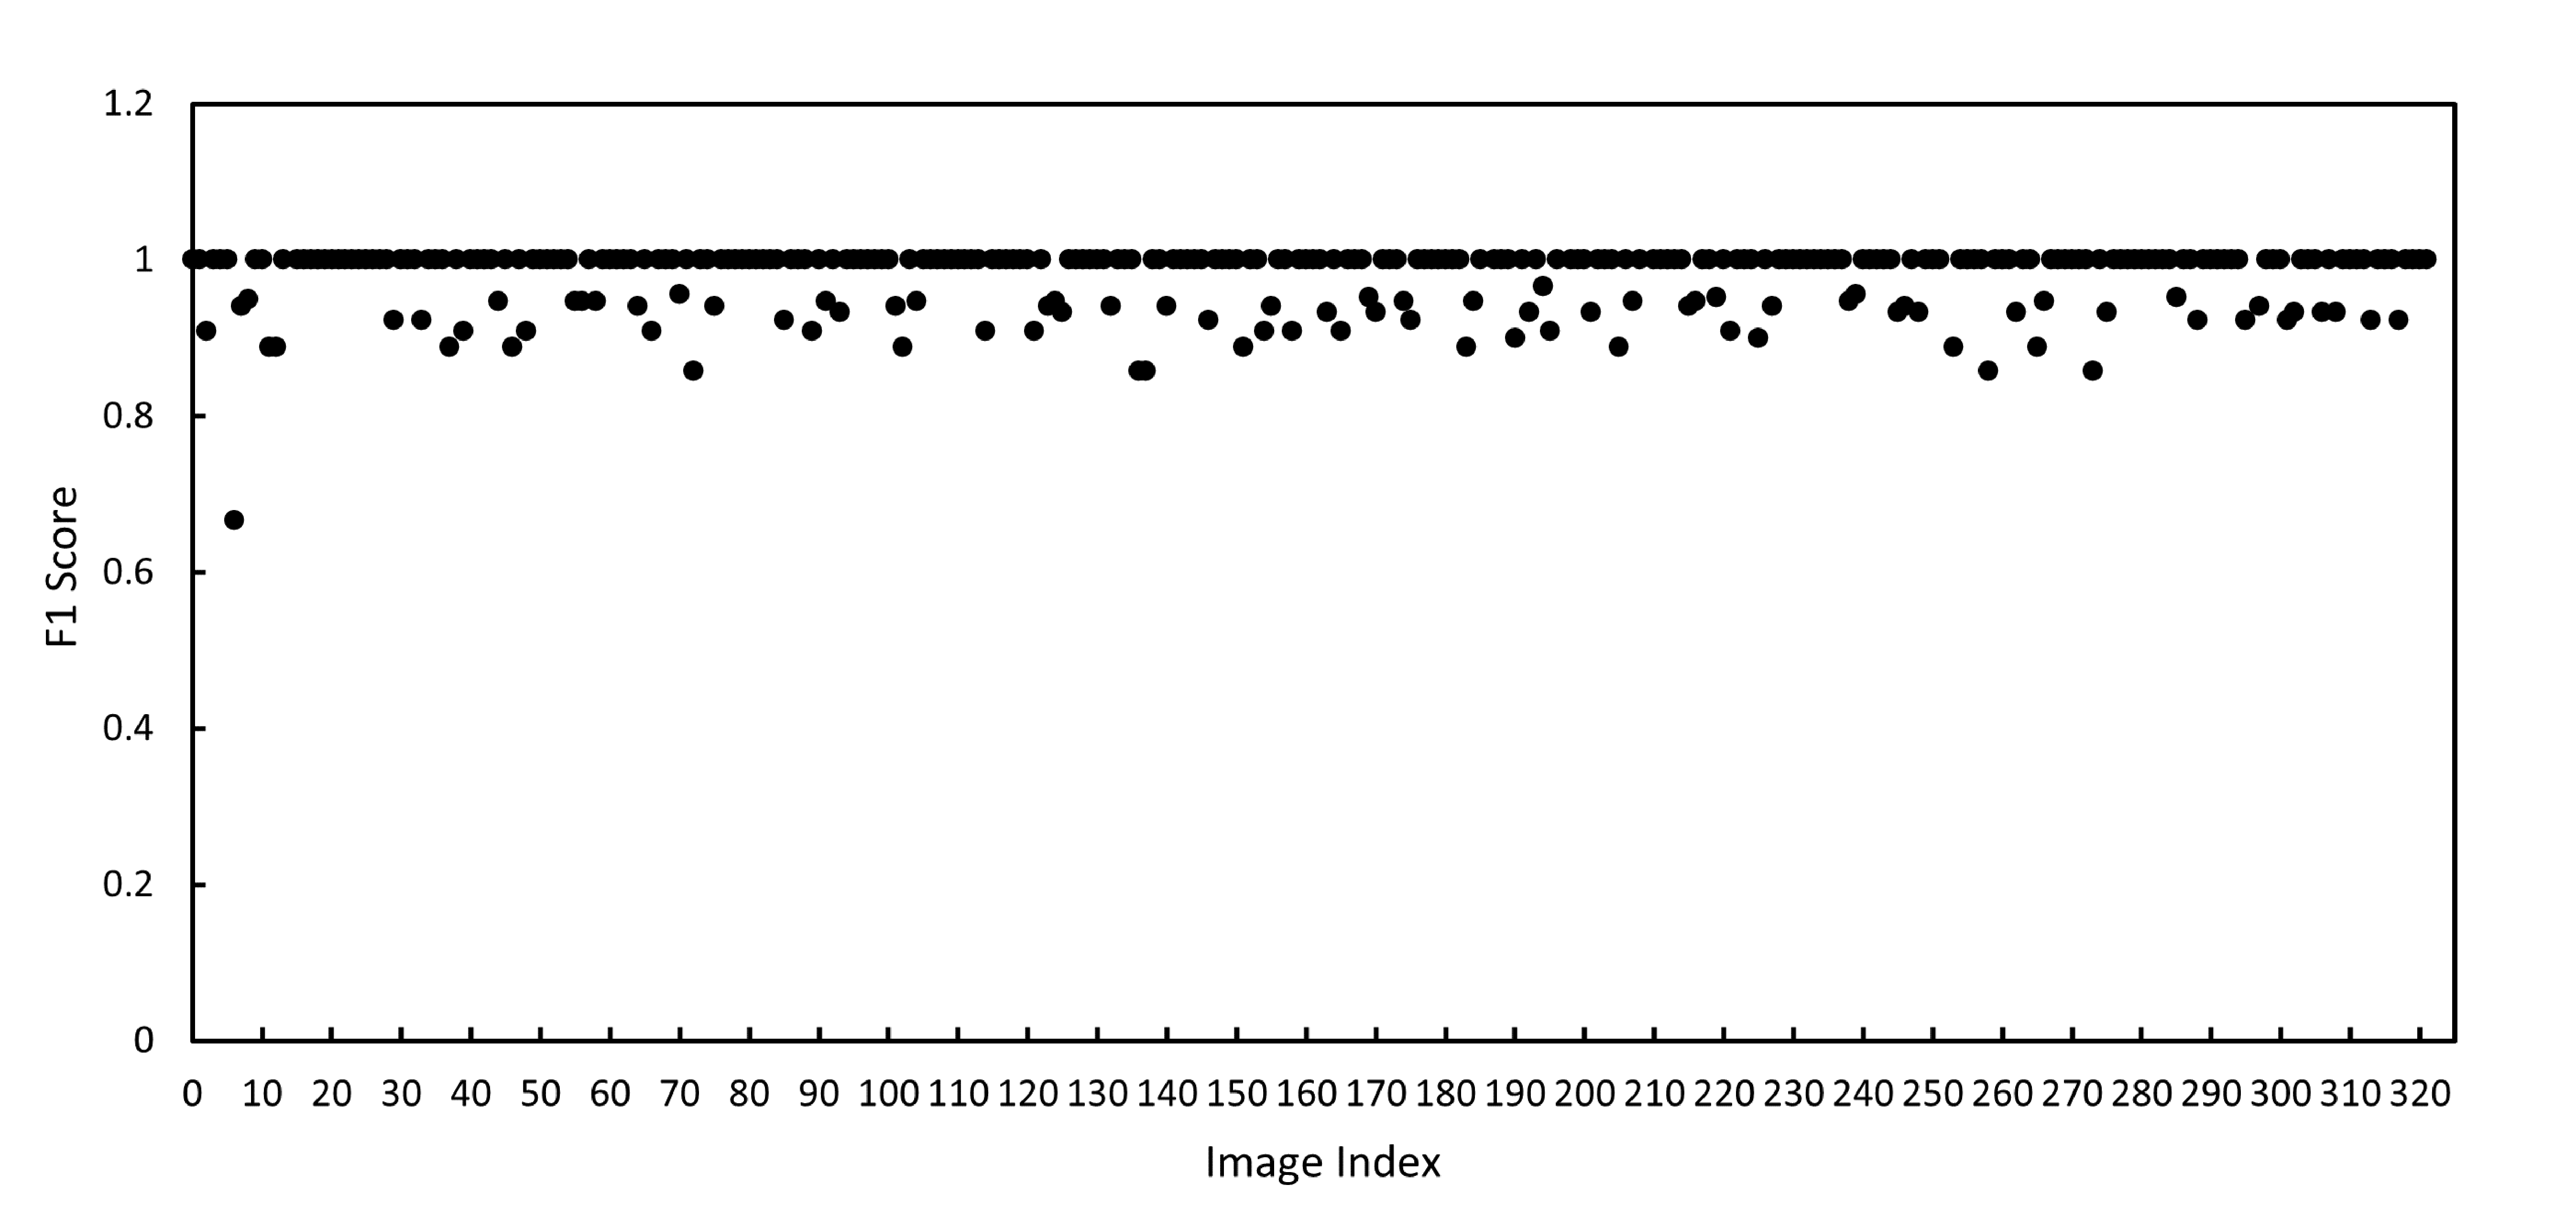
\includegraphics[width=\textwidth]{project_graphics/Fig8.eps}
	\caption{F1 Score vs Image Index Graph}
	\label{fig:fig8}
\end{figure}
The Receiver Operating Characteristic (ROC) curve was constructed by plotting the true positive rate (Recall) against the false positive rate (FPR) at various classification thresholds. For best-performing algorithms, the top-left corner of the graph would be touched by a ROC curve.
Here it was achieved as shown in \autoref{fig:fig9}
\par
\FloatBarrier
\begin{figure}[h]
	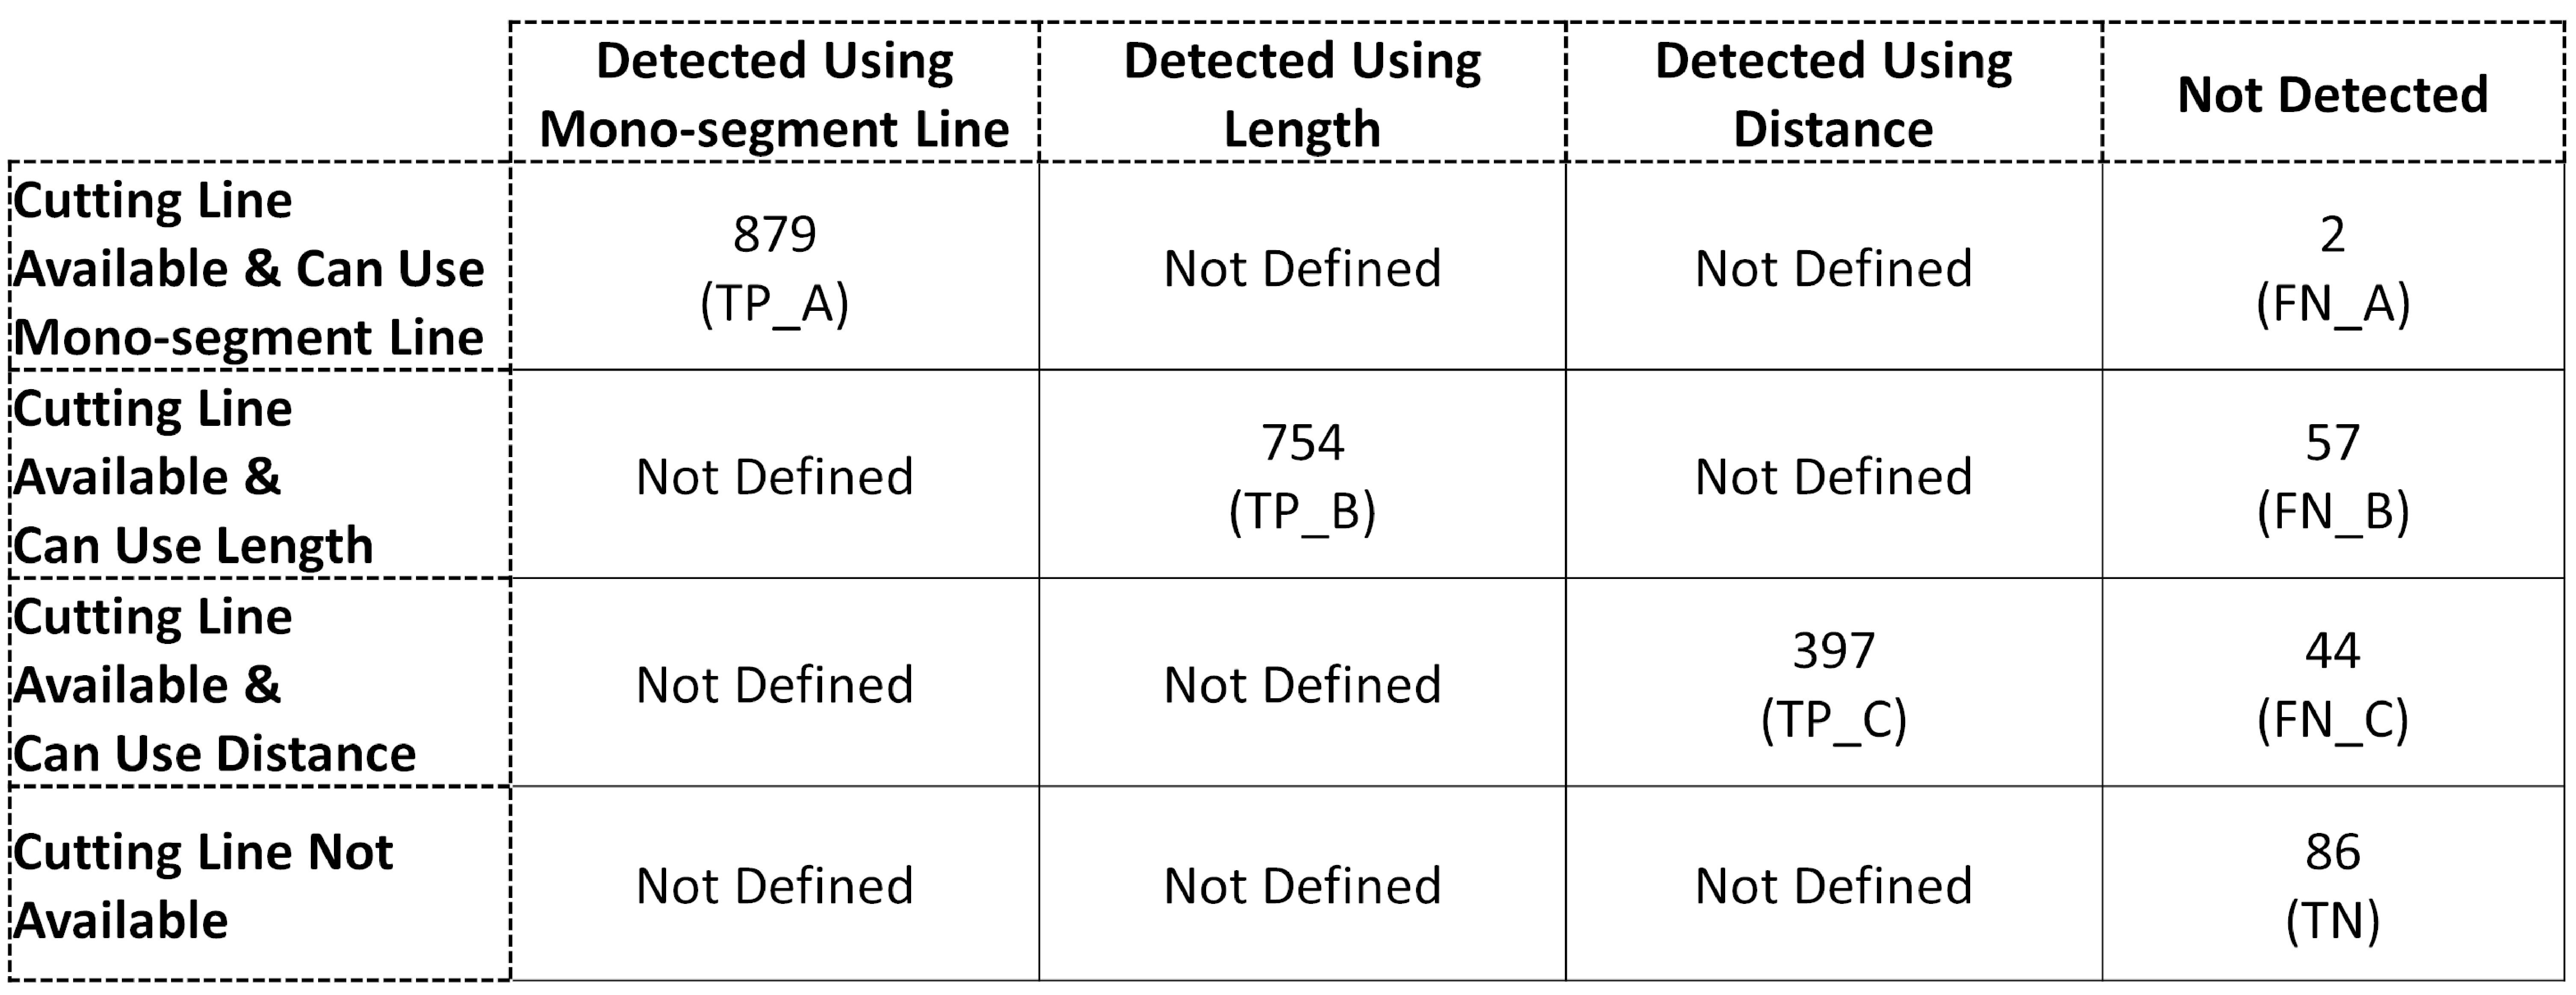
\includegraphics[width=\textwidth]{project_graphics/Fig9.eps}
	\caption{ROC Curve}
	\label{fig:fig9}
\end{figure}
\par
In summary, the algorithm's reliability and effectiveness in classification tasks are signified by the high F1 score, accuracy, and precision values. Furthermore, the perfect sensitivity suggested by the straight line in the ROC curve and the absence of false negatives further affirms the strong performance of the algorithm.
\par
\section{Efficiency Analysis of the Algorithm}

The efficiency analysis of the algorithm is based on the processing time of the algorithm. As mentioned in the methodology, there are main three sections in this algorithm. But for the efficiency analysis, time spent on preprocessing and the feature extraction were combined into one single section and called “initial preparation time”. Then time spent for the classification step was divided into three sections “single line detection”, “detection based on the size” and “detection based on the distance”. To measure the processing time, the Python library “timeit” was used.
\par
Based on the results, the most time-consuming area in the algorithm was identified as the preprocessing and the feature extraction area. Initially, processing time was compared by changing the hardware configurations. For this, two completely different computers were used to run the program and capture the processing time as shown in the \autoref{tab:tab2}. 1st configuration was Intel Core i5 - 9300H CPU @ 2.40GHz Processor (9th Gen), 16.0 GB RAM, 512 GB SSD Harddisk, and 2nd configuration was Intel Core i5 - 4210U CPU @ 1.70GHz Processor (4th Gen), 8 GB RAM, 750 GB SATA Harddisk.
\par
\FloatBarrier
\begin{table}[h]
\begin{tabular}{crl}
\hline
Configuration & Min Proc. Time (ms) & Max Proc. Time (ms)\\\hline
1st configuration & 66.42  & 716.73 \\
2nd configuration & 103.24 & 2078.21 \\\hline
\end{tabular}
\caption{Performance of the Algorithm}
\label{tab:tab2}
\end{table}
According to the \autoref{tab:tab2}, a huge contrast in the processing time was noticed. The CPU is responsible for executing instructions and performing calculations. The 1st computer has a higher clock speed (2.40GHz) compared to the 2nd computer. A higher clock speed generally means faster processing, Therefore, one reason for the less processing time in the 1st computer is CPU performance. Other factors such as the number of cores and the microarchitecture also play a role. 
\par
In the computer architecture, RAM is used to store data that the CPU needs to access quickly. Having more RAM allows this kind of complex algorithm to be processed efficiently. The first laptop has 16GB of RAM, which is twice the capacity of the second laptop's 8GB. This means that the first laptop can handle larger amounts of data in memory, potentially leading to faster algorithm execution.
\par
The storage drive, whether it's an SSD or an HDD, affects the algorithm's speed primarily during data read/write operations like loading JSON file etc. SSDs are generally faster than traditional HDDs, offering quicker data access times. The first laptop's 512GB SSD is likely to provide faster read/write speeds compared to the second computer's 750GB SATA drive. Therefore, the 1st computer was taken into further processing. 
\par
When further analyzing the preprocessing and feature extraction stages, a hypothesis was formulated to examine the impact of the number of neighboring plant section combinations in a sample image on the efficiency of the algorithm. The relationship between these two parameters was investigated using Big O notation, a mathematical notation commonly used in computer science. Big O notation, denoted as O(f(n)), where "O" represents the order of growth and "f(n)" denotes the algorithm's growth rate as a function of the input size "n," was employed to analyze and compare algorithm performance as the input size increased. Typically, the function "f(n)" represents the worst-case time complexity of the algorithm, providing a clear indication of its efficiency and scalability with increasing input size.
\par
Based on the algorithm's performance behavior in relation to the input size, various types of Big O notations have been defined. For instance, O(1) represents constant performance, O(log n) denotes logarithmic performance, and O(n) signifies linear performance. Considering the processing structure of this algorithm, it was theoretically assumed that the algorithm's Big O notation complexity should be linear (O(n)). To validate this assumption, a graph was plotted, as depicted in \autoref{fig:fig10}, representing the algorithm's processing time against the number of neighboring plant section combinations. The graph was examined to identify patterns in the growth of the processing time.
\par
\FloatBarrier
\begin{figure}[h]
	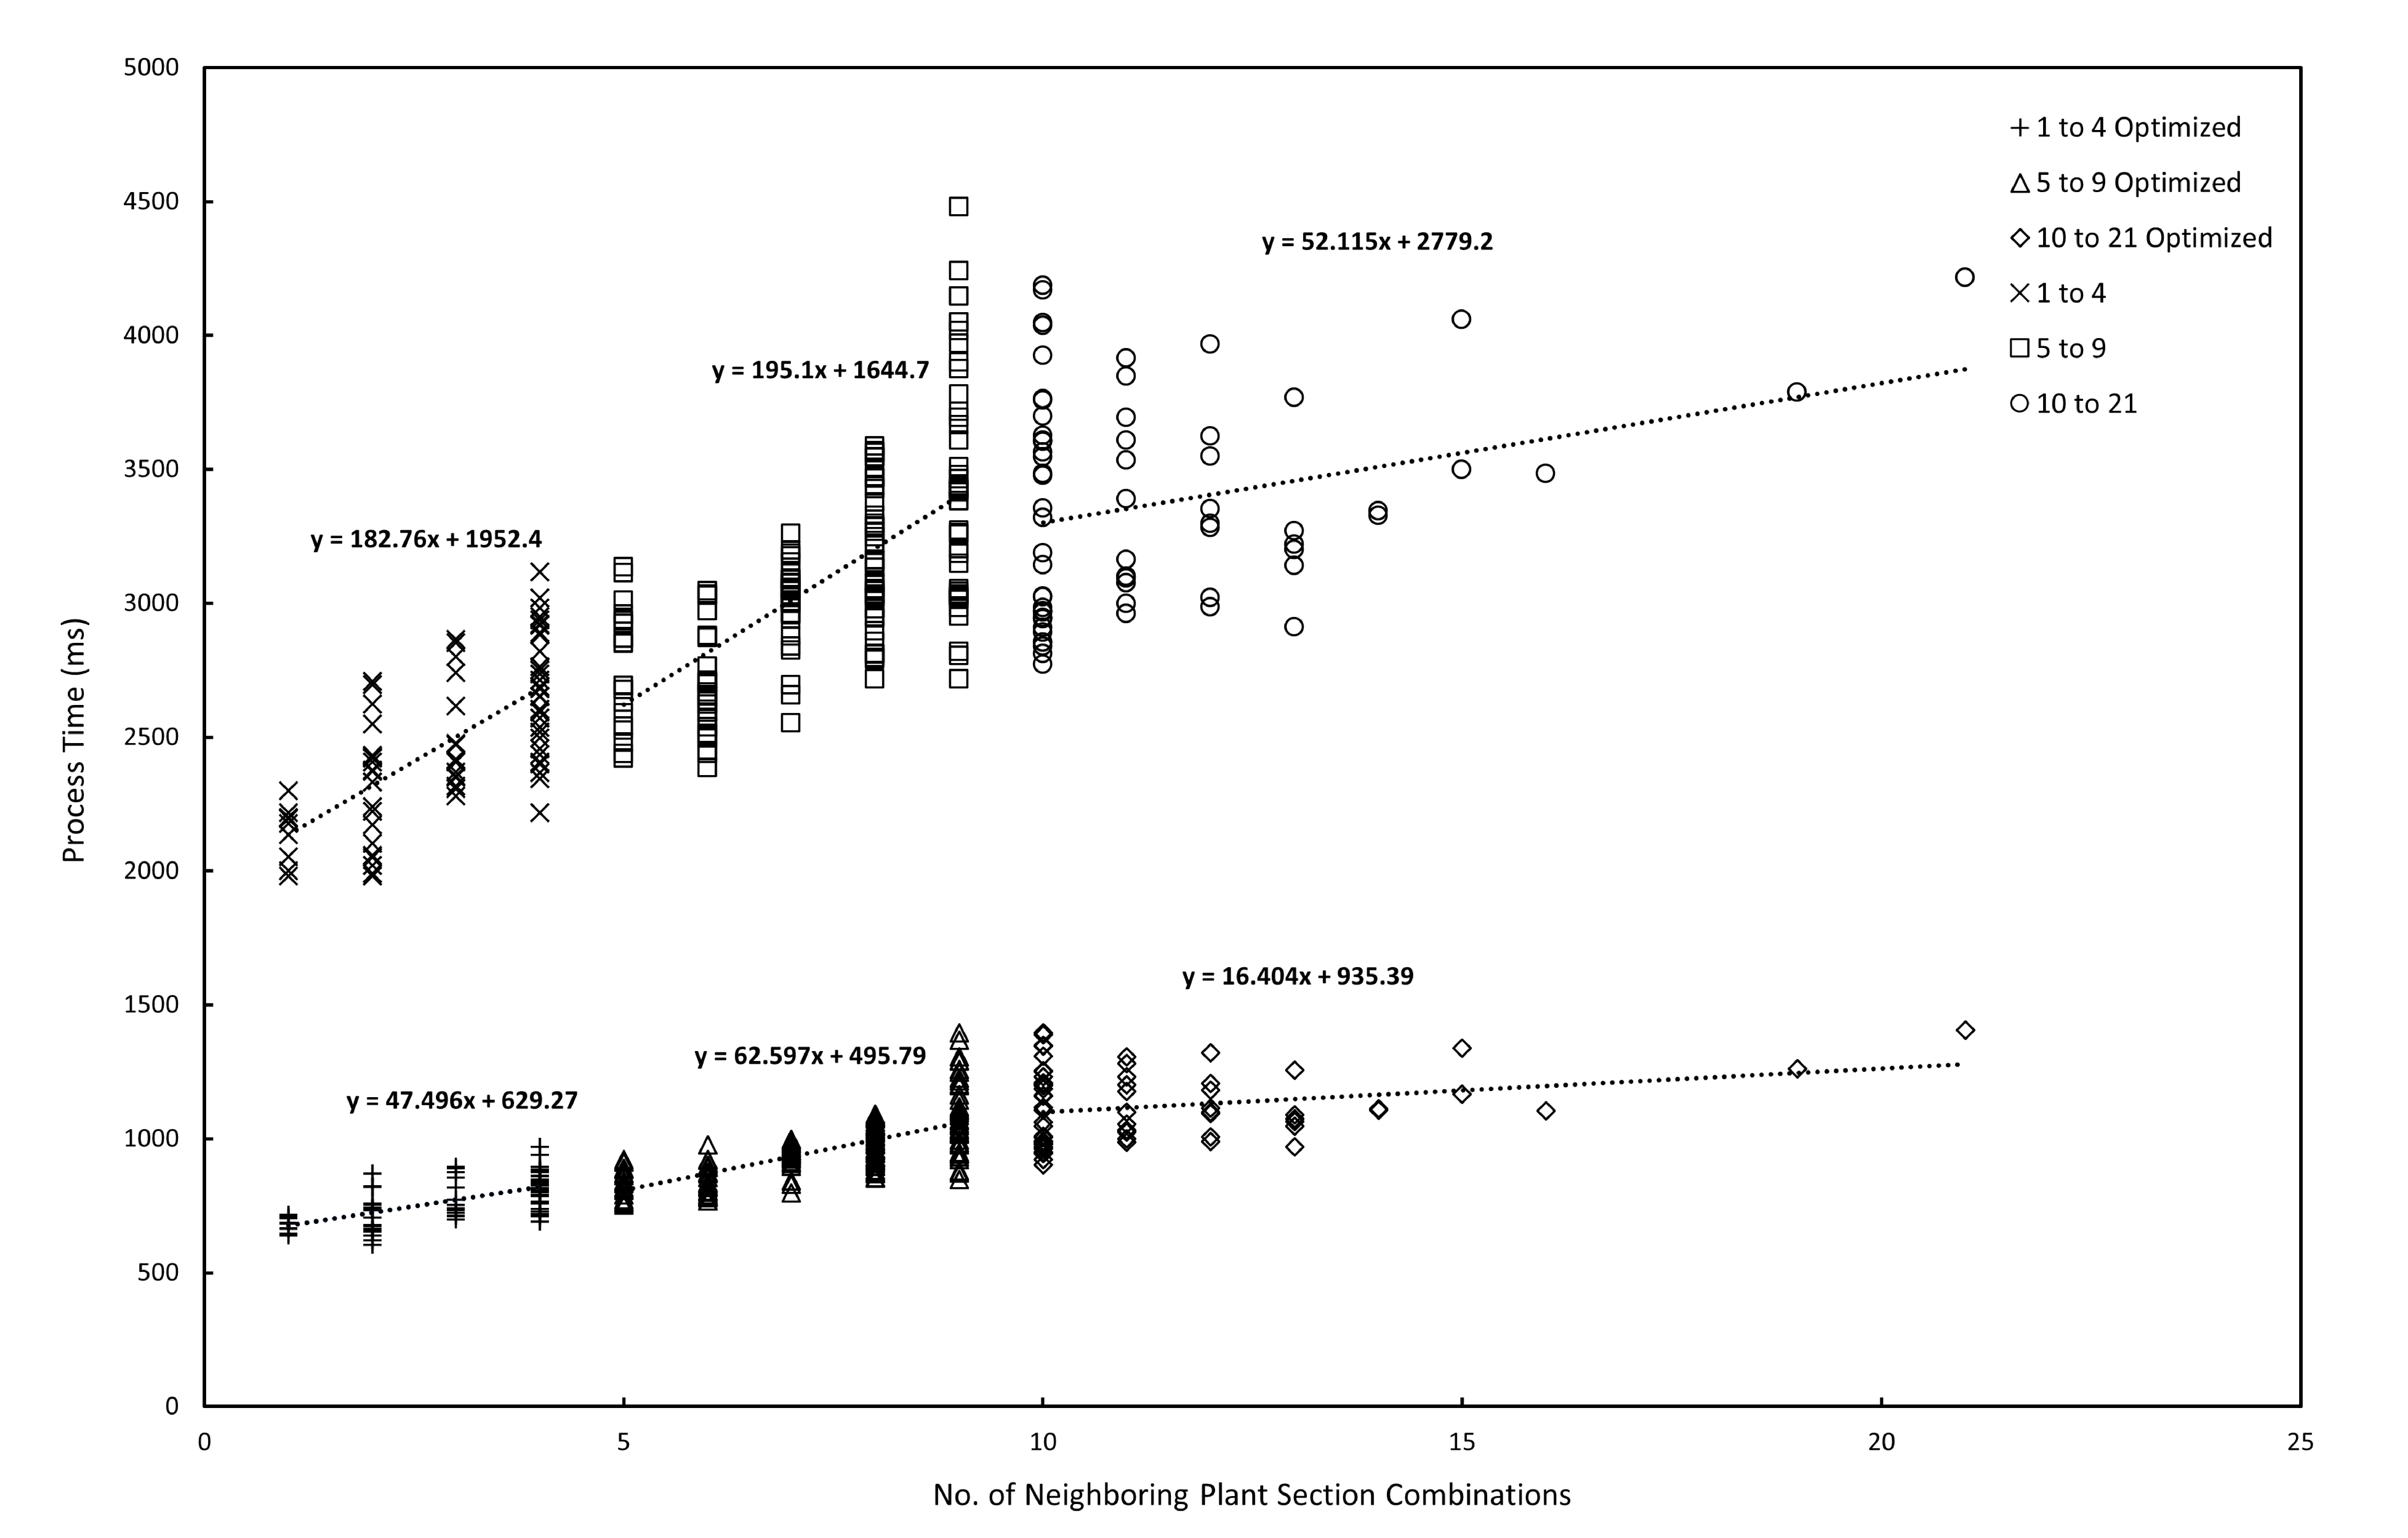
\includegraphics[width=\textwidth]{project_graphics/Fig10.eps}
	\caption{Process Time vs No. of Neighboring Plant Section Combinations }
	\label{fig:fig10}
\end{figure}
Based on the algorithm's performance behavior in relation to the input size, various types of Big O notations have been defined. For instance, O(1) represents constant performance, O(log n) denotes logarithmic performance, and O(n) signifies linear performance. Considering the processing structure of this algorithm, it was theoretically assumed that the algorithm's Big O notation complexity should be linear (O(n)). To validate this assumption, a graph was plotted, as depicted in \autoref{fig:fig10}, representing the algorithm's processing time against the number of neighboring plant section combinations. The graph was examined to identify patterns in the growth of the processing time. Additionally, to compare the algorithm's performance, a processing time reduction technique utilizing the external contour detection method(optimized) (refer to subtopic 2.2) instead of the internal contour detection method (utilizing the whole solid section of the plant) was employed as shown in the \autoref{fig:fig10}
\par
Observing \autoref{fig:fig10}, significant differences in the growth rate of the processing time (gradient) were noticed as the number of combinations increased. The relevant Big O notation or the relationship between the number of combinations and the processing time was summarized in the \autoref{tab:tab3}. This observation can be attributed to the fact that as the number of combinations increases in an image, the size of the plant decreases, including both the plant's section size and the size of the outside contour. Consequently, less time is required for processing the contours. This is further explained in the following graph. (See \autoref{fig:fig11}). 
\par
\FloatBarrier
\begin{table}[h]
\begin{tabular}{crl}
\hline
Range of Combinations & Relationship\\\hline
1 to 4 Not Optimized & O(n) = 182.76n + 1952.4 \\
5 to 9 Not Optimized & O(n) = 195.1n + 1644.7 \\
10 to 21 Not Optimized & O(n) = 52.115n + 2779.2 \\
1 to 4 Optimized & O(n) = 47.496n + 629.27 \\
5 to 9 Optimized & O(n) = 62.597n + 495.79 \\
10 to 21 Optimized & O(n) = 16.404n + 935.39 \\\hline
\end{tabular}
\caption{Big O Notation ( "O(n)" represents processing time and "n" represents No. of combinations)}
\label{tab:tab3}
\end{table}
\par
\FloatBarrier
\begin{figure}[h]
	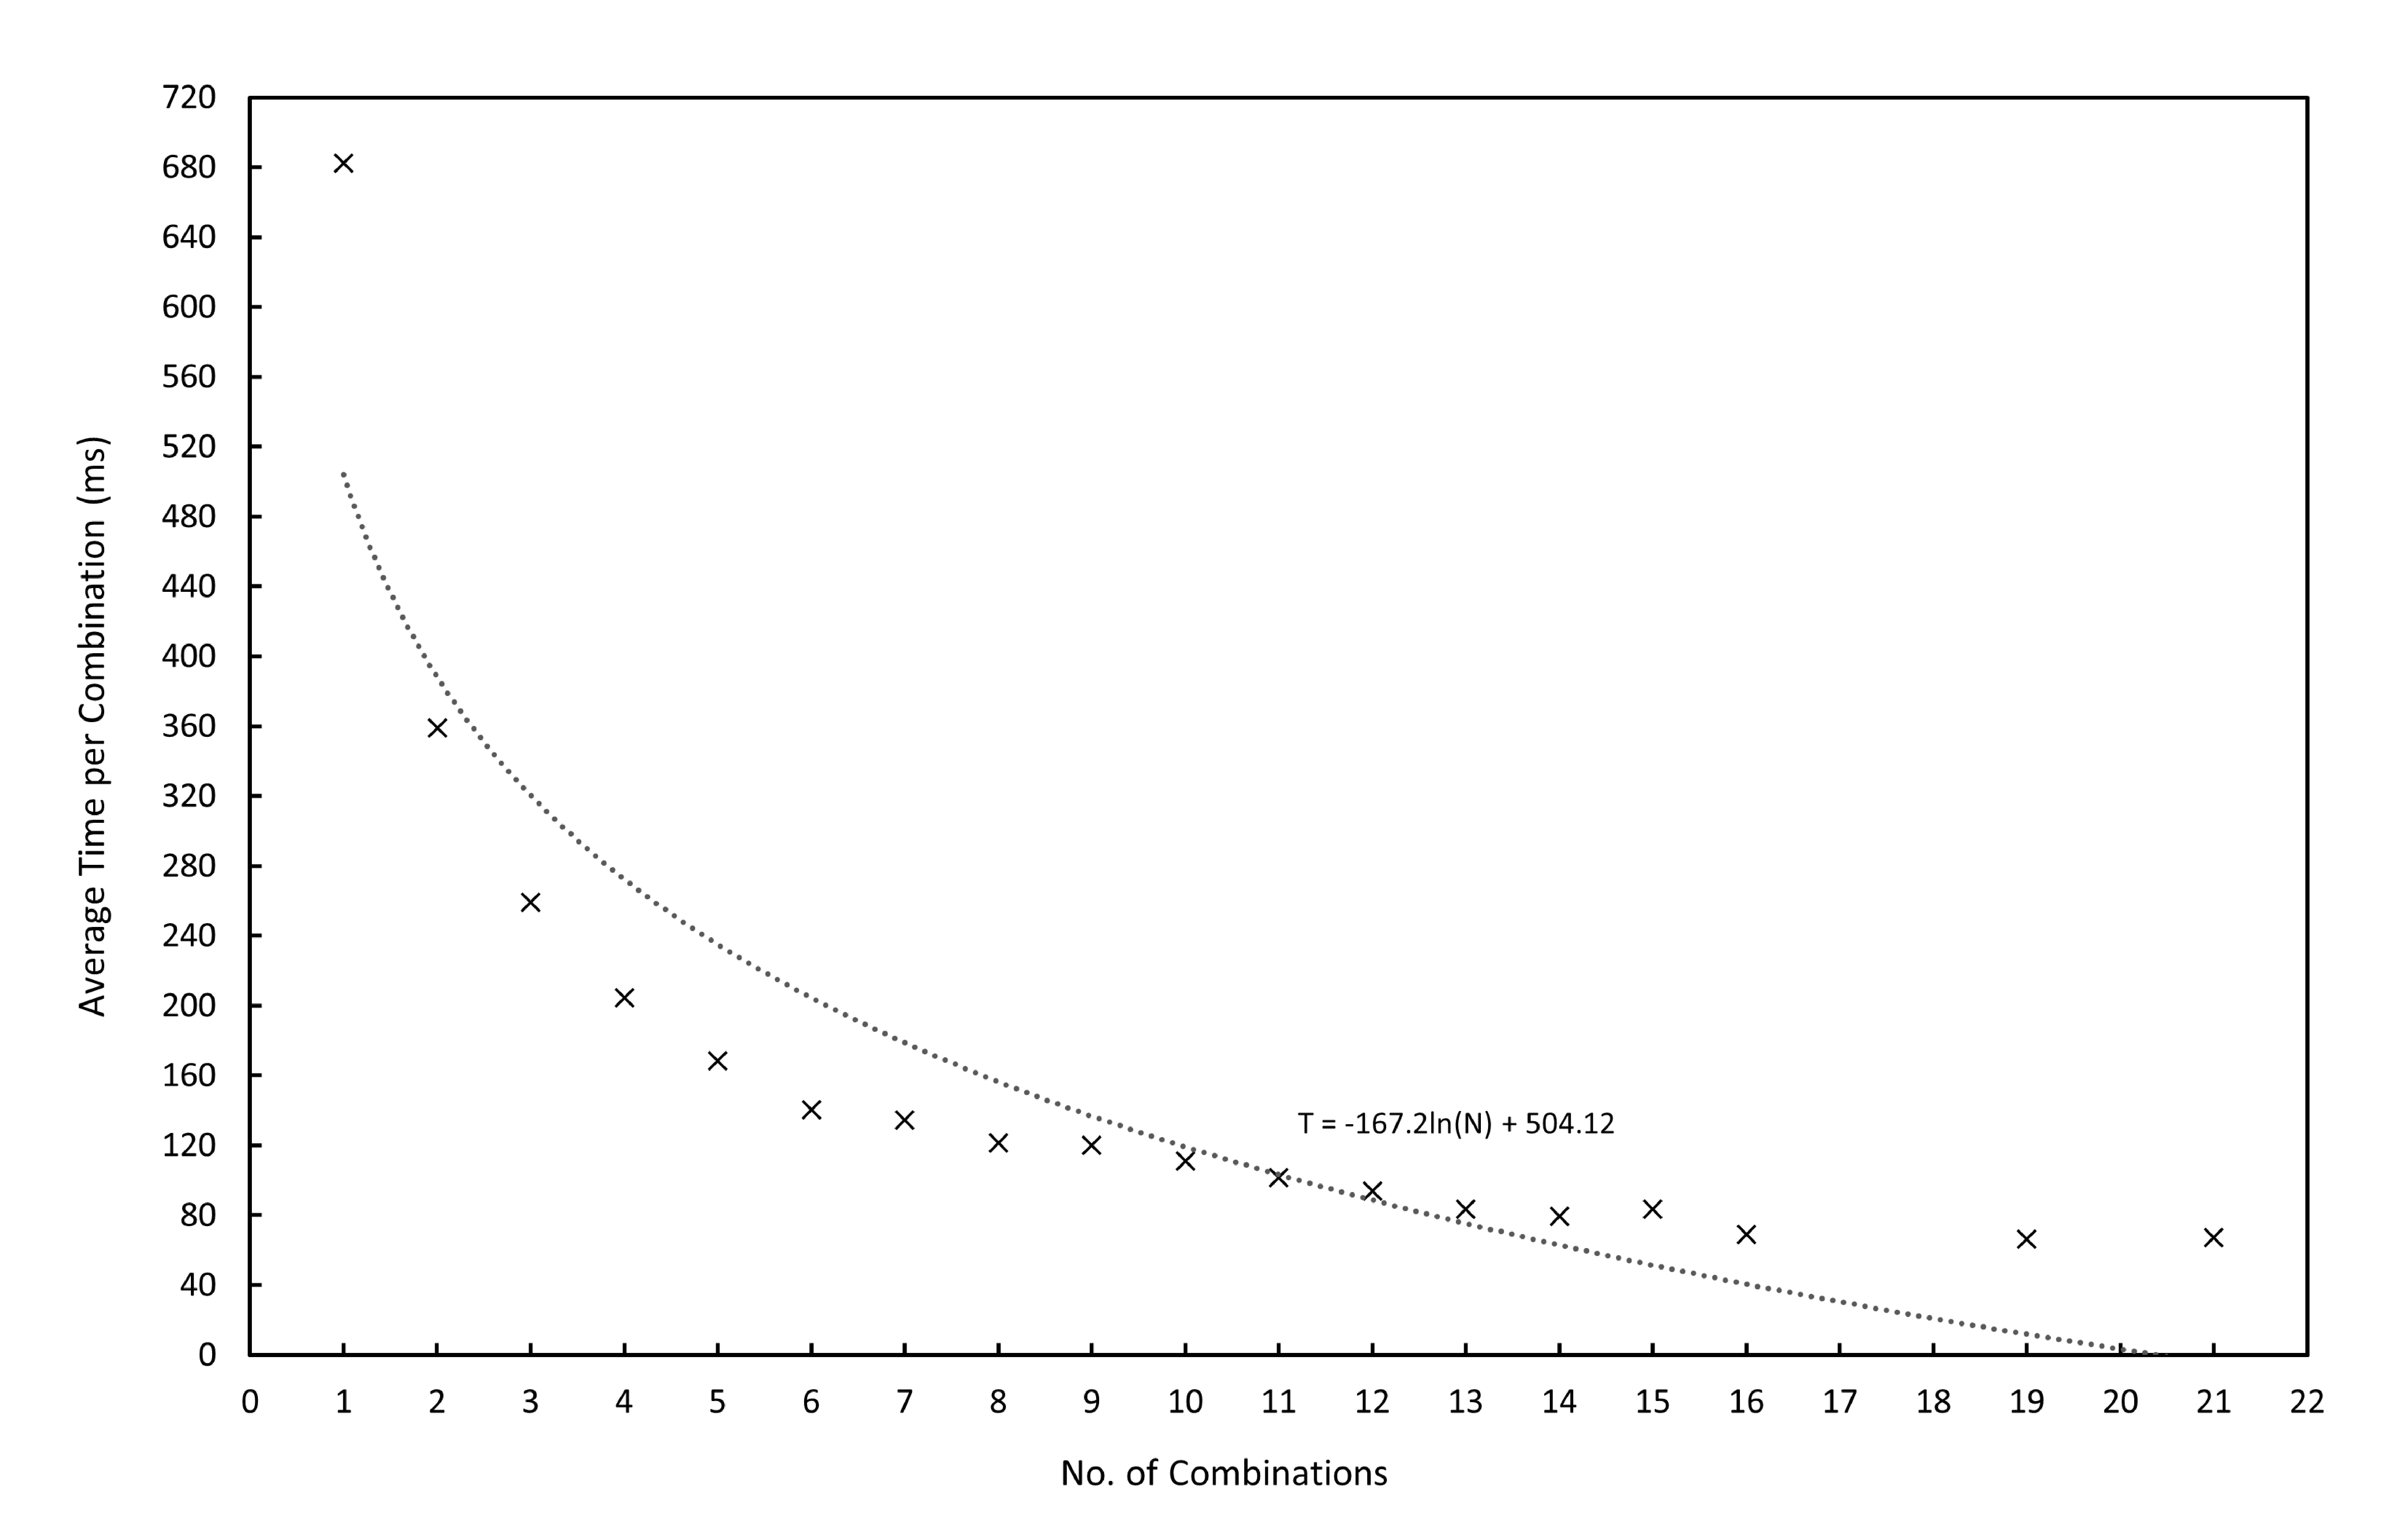
\includegraphics[width=\textwidth]{project_graphics/Fig11.eps}
	\caption{Average Time per Combination vs No. of Neighboring Plant Section Combinations }
	\label{fig:fig11}
\end{figure}
Also, a logarithmic relationship was found in the average time per combination vs No. of combinations. 
\par
\FloatBarrier
\begin{align}
\intertext{"T" represents the average time per combination and "N" represents the number of combinations(N>0)}
T &=-167.2ln(N)+504.12
\end{align}
Also based on the optimized algorithm utilizing the external contour detection method, roughly 3 times the processing time reduction was achieved due to less amount pixels available on the external contour compared to the whole solid section of the plant.
\par
The histogram presented the duration allocated to the classification step. A visual representation of single-line detection is provided in \autoref{fig:fig12}, where the histogram illustrates a left-skewed distribution. This signifies that the range of time dedicated to detecting a single line span from 39ms to 239ms.
\par
\FloatBarrier
\begin{figure}[h]
	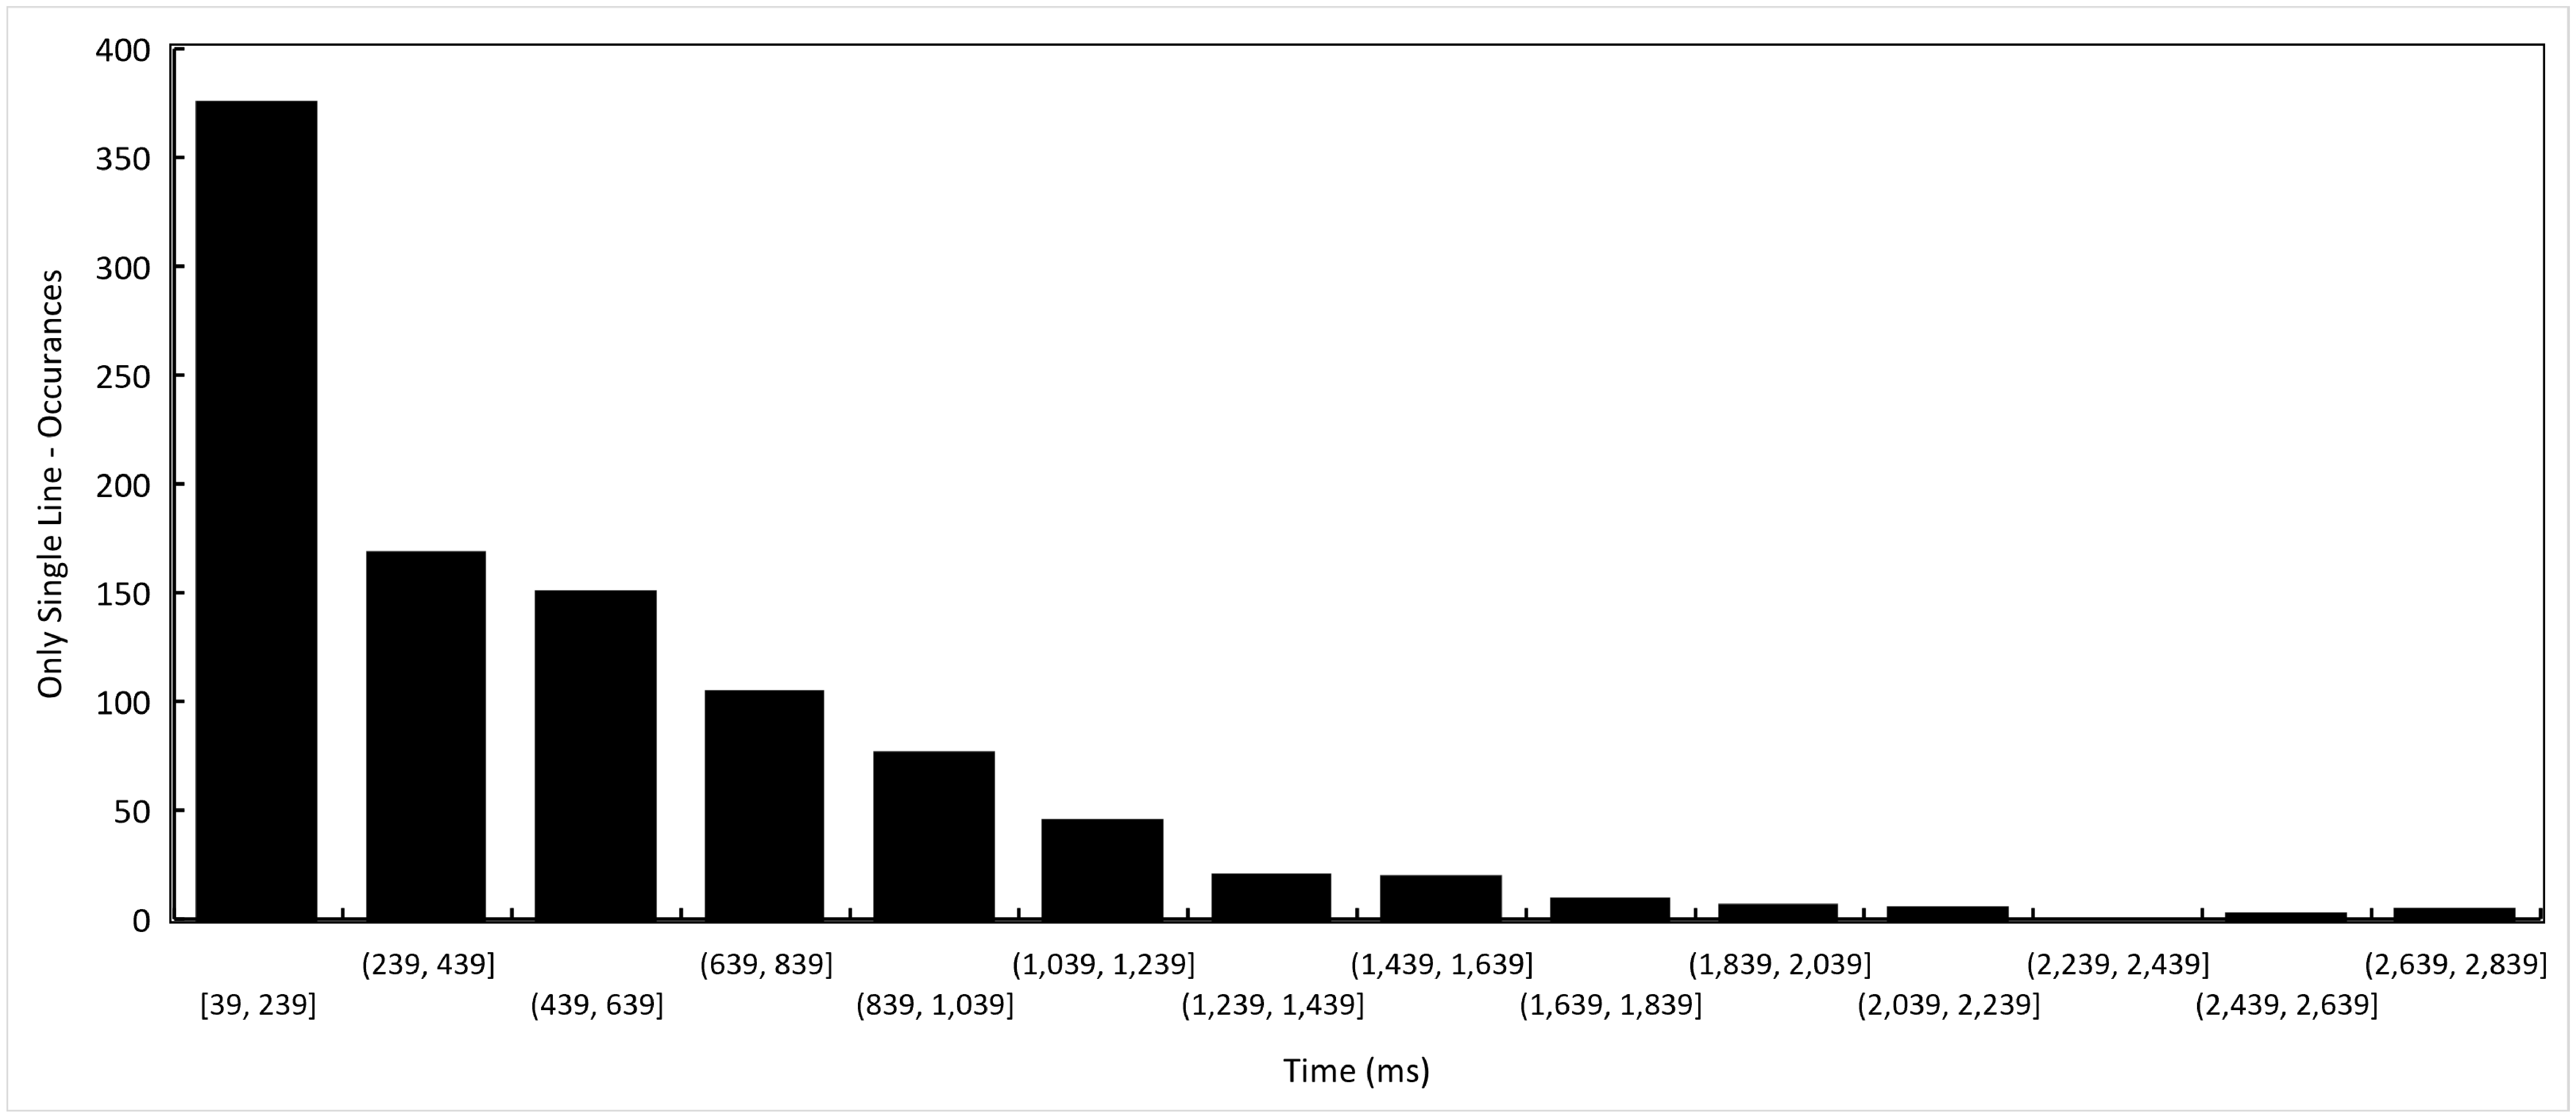
\includegraphics[width=\textwidth]{project_graphics/Fig12.eps}
	\caption{Histogram - Detection using Only Single Line  }
	\label{fig:fig12}
\end{figure}
\par
With respect to detection based on size, as depicted in\autoref{fig:fig13}, the time distribution follows a similar left-skewed pattern. Comparable to the previous instance, the duration for this type of detection also lies in a similar range, that is, between 41ms to 241ms.
\par
\FloatBarrier
\begin{figure}[h]
	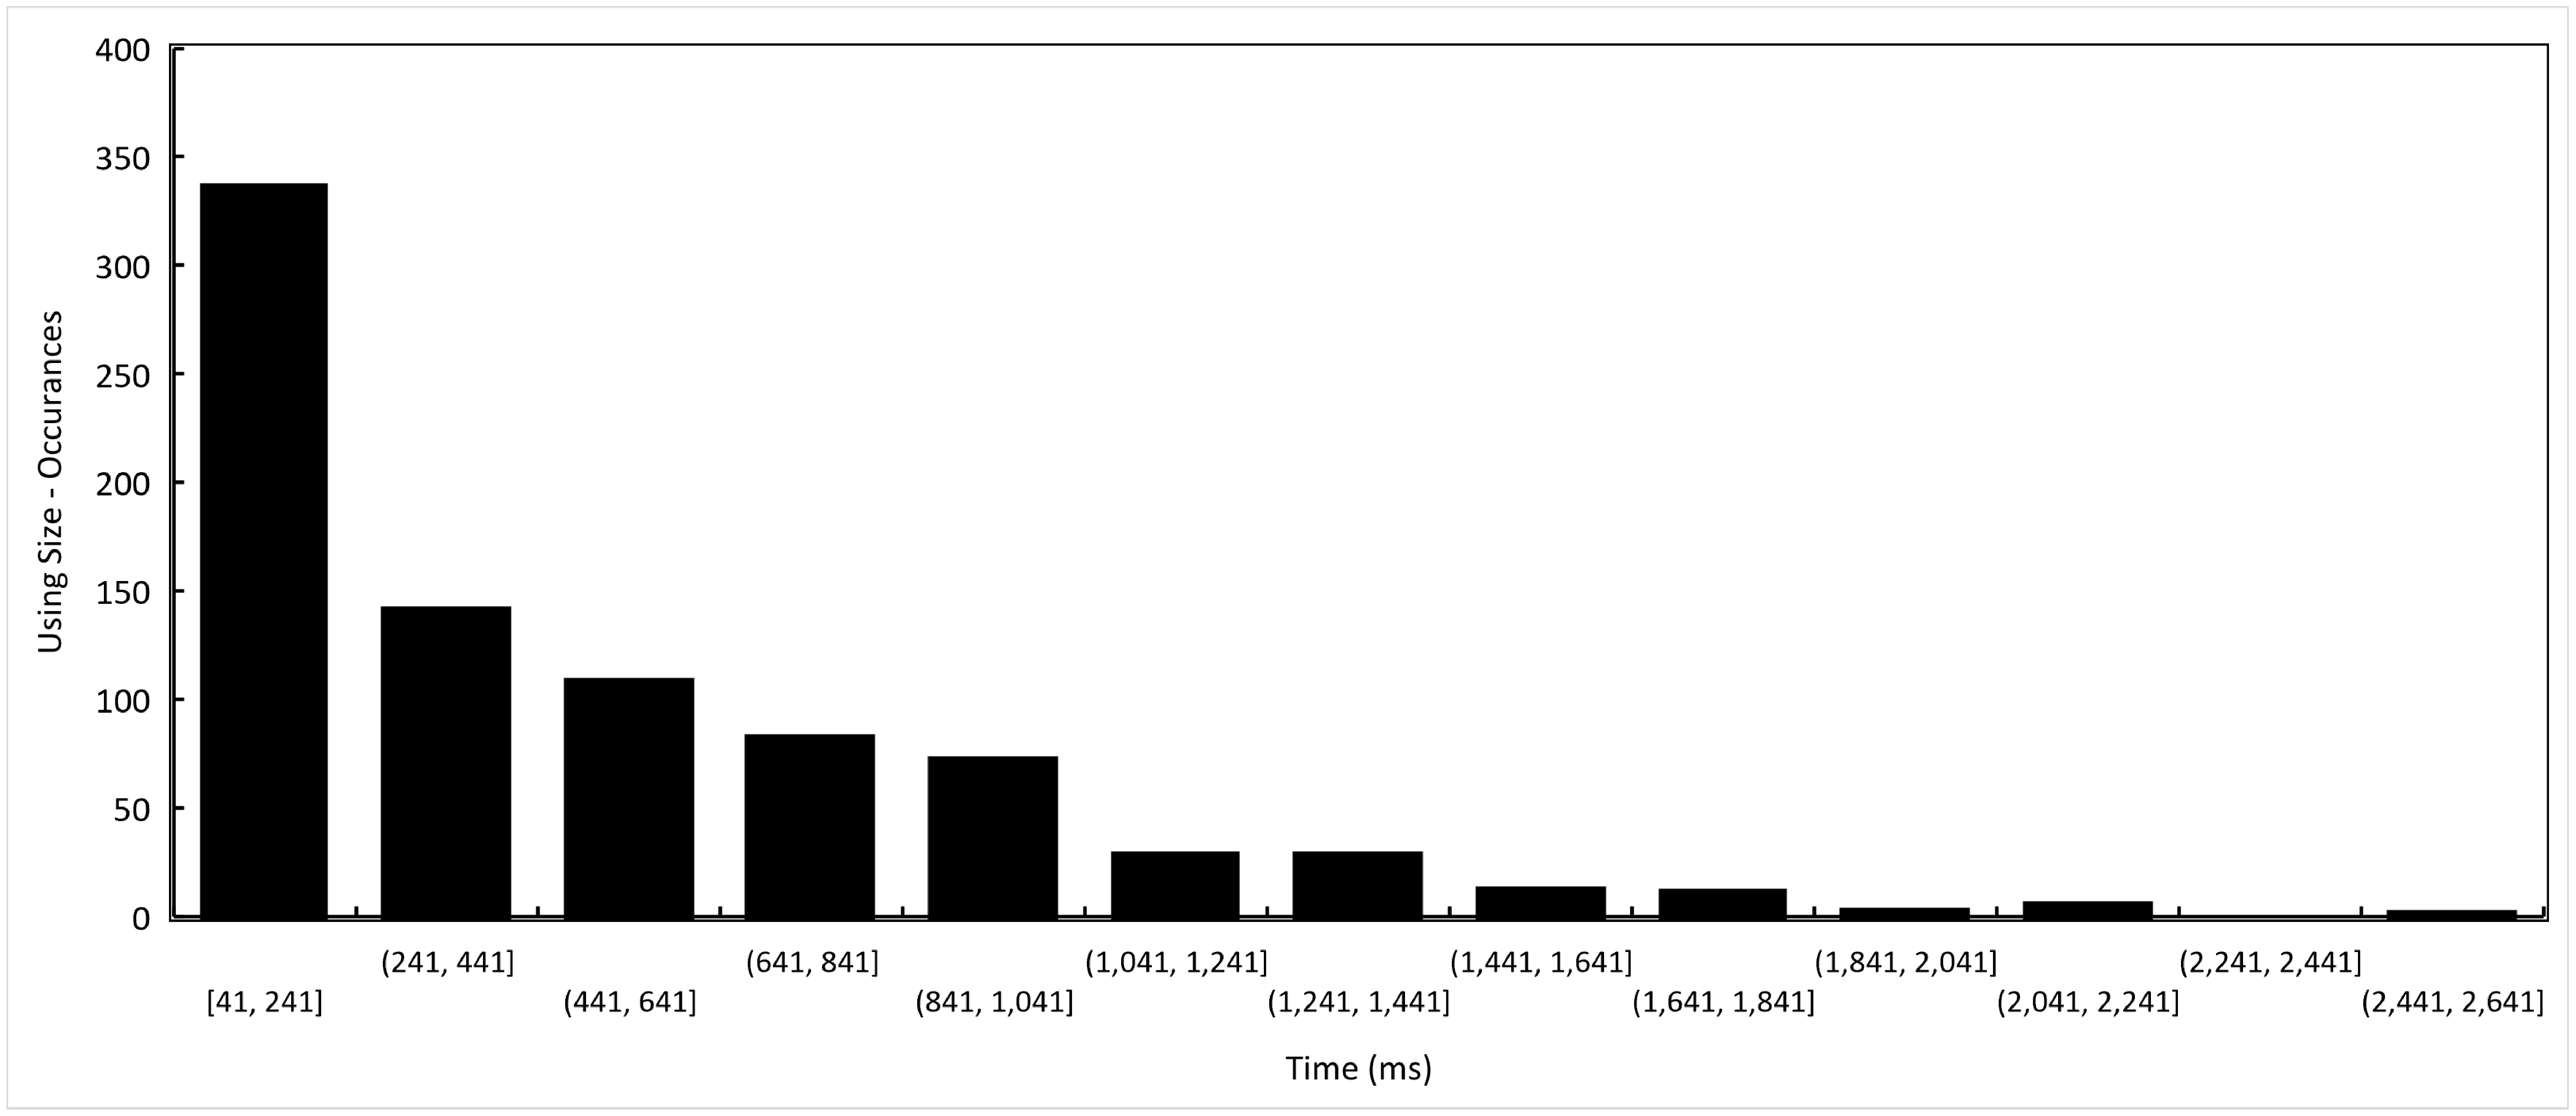
\includegraphics[width=\textwidth]{project_graphics/Fig13.eps}
	\caption{Histogram - Detection using Size  }
	\label{fig:fig13}
\end{figure}
\par
However, a deviation can be observed when we examine the time spent for detection based on distance, as represented in \autoref{fig:fig14}. In this particular scenario, the duration is slightly increased, ranging from 286ms to 486ms, which is higher than the time required for the other two forms of detection.
\par
\FloatBarrier
\begin{figure}[h]
	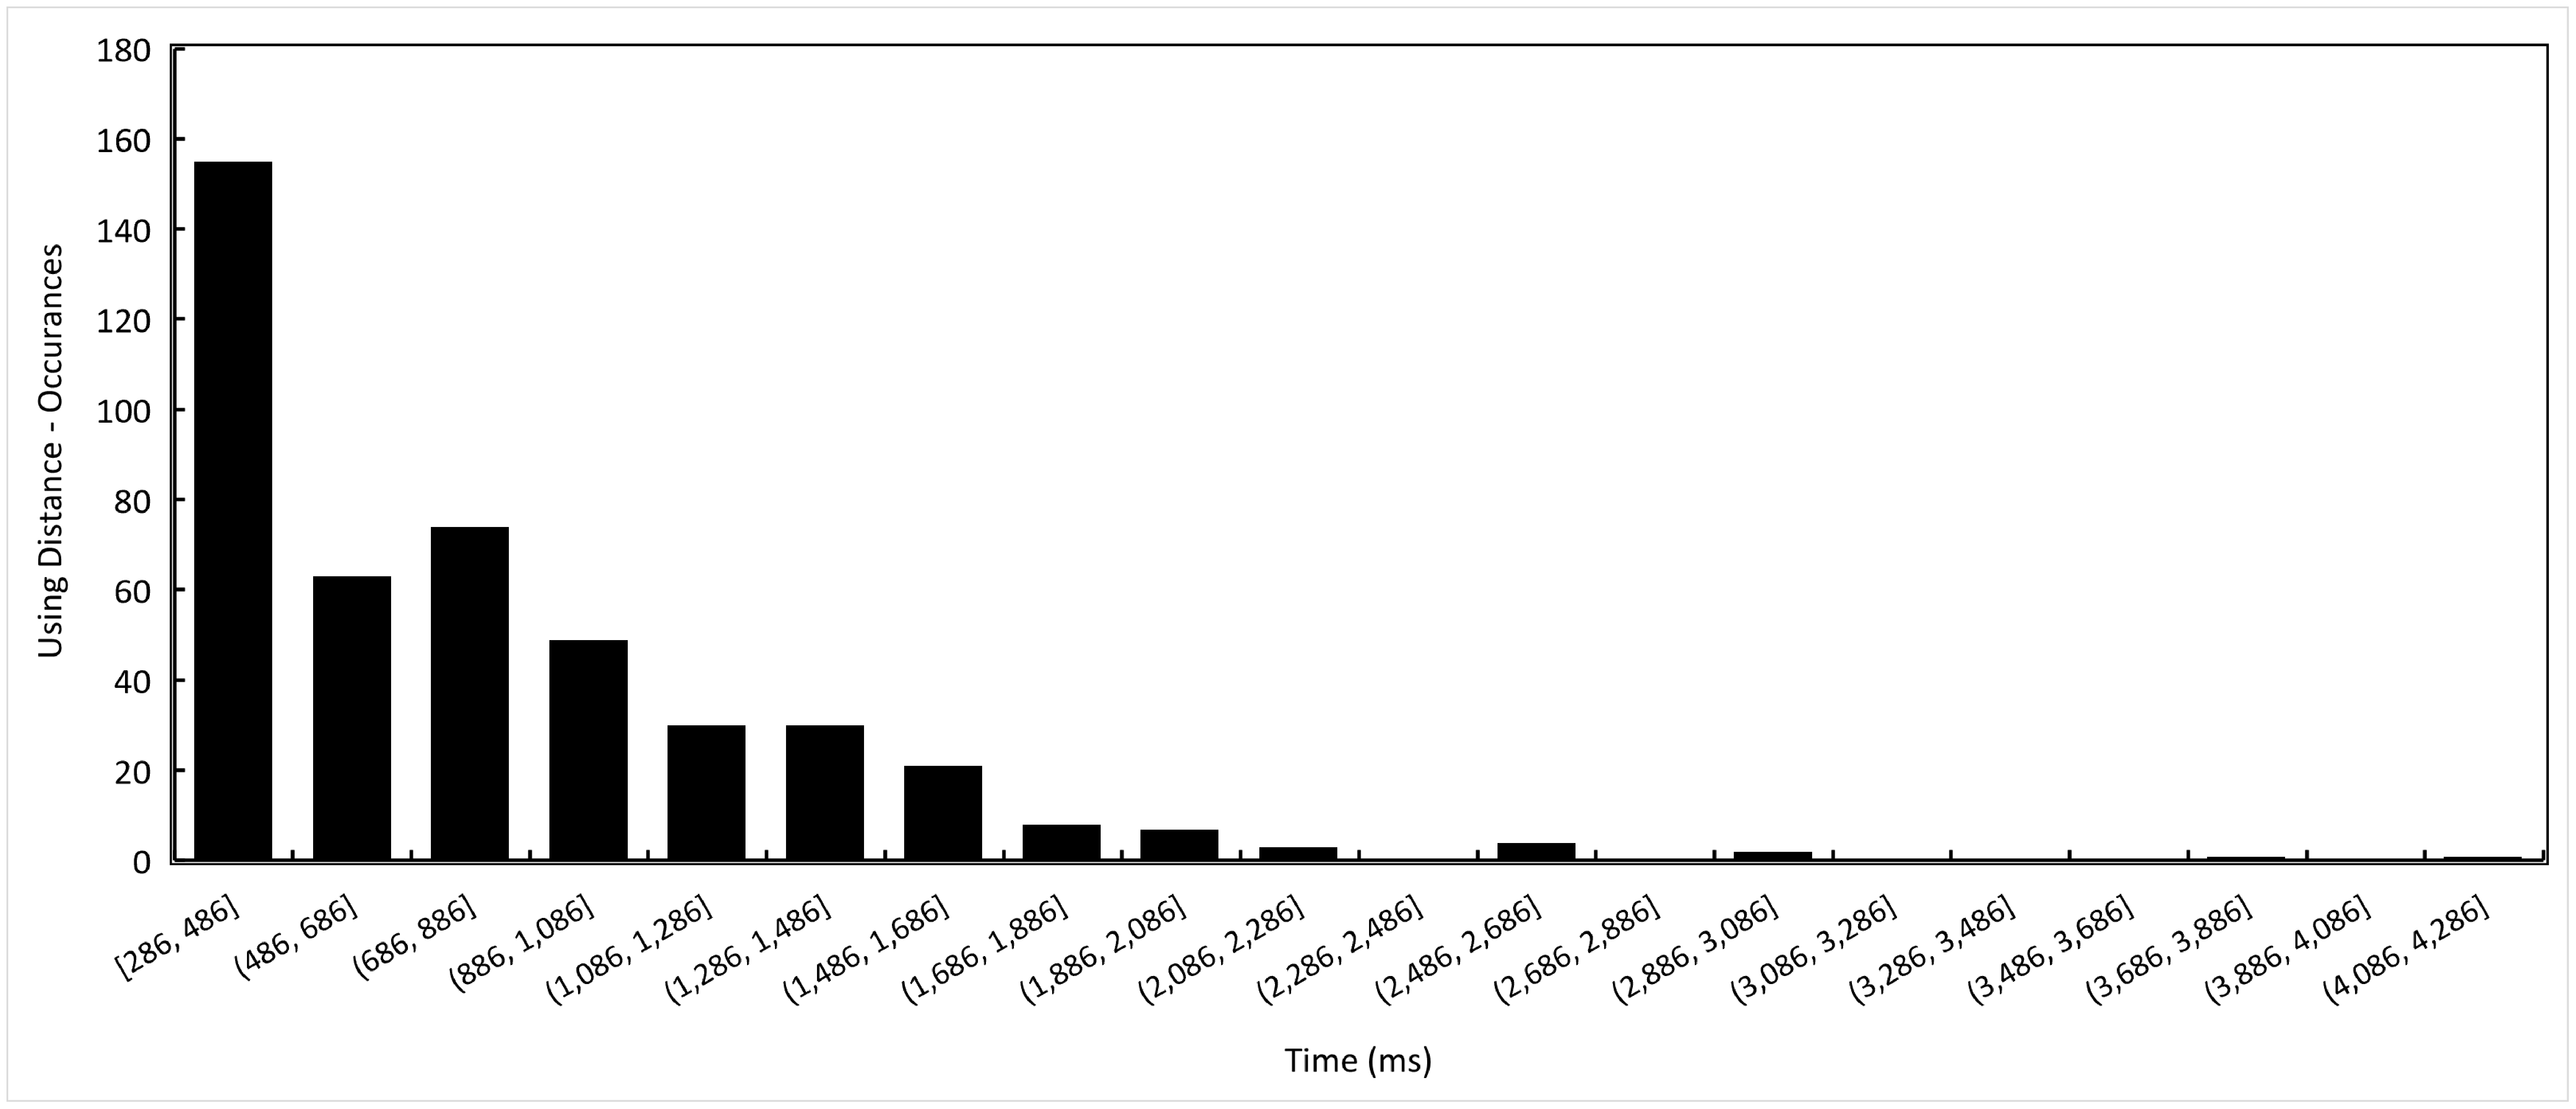
\includegraphics[width=\textwidth]{project_graphics/Fig14.eps}
	\caption{Histogram - Detection using Distance  }
	\label{fig:fig14}
\end{figure}
\par
Therefore, it can be interpreted from the histograms that while the time distributions for single-line detection and size-based detection are quite similar and relatively lower, the time required for distance-based detection is marginally greater.
\par
It may be worth considering whether the increased time for distance-based detection is due to the inherent complexity in this type of detection, or whether it could be optimized further. Finally understanding these factors could potentially inform decisions about which detection method needs to be more optimized in future development. 


\chapter{Basisbefehle im Textsatz / Basic Controls for Textset}
\section{Strukturieren von Dokumenten / Structure of Documents}
Im Folgend sind die Strukturebenen des Textsatzes von oben nach unten dargestellt.\\
The follows shows the structural levels of the text set top-down:

\boxed{
\begin{minipage}[]{\textwidth}
	\chapter*{Kapitel / Chapter}
	\section*{Abschnitt / Section}
	\subsection*{Unterabschnitt / Subsection}
	\subsubsection*{Unterunterabschnitt / Subsubsection}
	\paragraph{Absatz / Paragraph}
	\quad
\end{minipage}
}
Leerzeilen werden mit \textbackslash\textbackslash\space eingefügt, ein neuer Paragraph ohne Überschrift mit \textbackslash par.\\
To insert a newline type \textbackslash\textbackslash, a new paragraph without title is set with \textbackslash par.

\section{Gleichungen / Equations}
Für das Darstellen von Gleichungen das amsmath-Paket verwenden, z.B. mithilfe der align-Umgebung:\\
Use the amsmath-package for equations, for example the align-environment:
\begin{lstlisting}
\begin{align}
	S(s)&=1-T(s)

	T(s)&=\frac{GK(s)}{GK(s)+1}
\end{align}
\end{lstlisting}
Ergebnis / Result:\par
\begin{align}
	S(s)&=1-T(s)
	\intertext{Beispielgleichung}
	T(s)&=\frac{GK(s)}{GK(s)+1}
\end{align}

Für Einheiten das siunitx-Paket benuten. Z.B.: $v$ in $\si{\m\per\s}$\\
Use the siunitx-package for unit typesetting. E.g.: $v$ in $\si{\m\per\s}$\par
\section{Grafiken / Graphics}
Wenn möglich, Vektorgrafiken verwenden und schwarz/weiß kompatible Grafiken erstellen. Grafiken in figure-Umgebung einbetten. Anstelle die Position mit der Option [h!] oder [H] zu verändern, bis zum Abschluss des Dokumentes warten und, falls noch immer notwendig, mit Clearpage arbeiten oder mit FloatBarrier erzwingen. Im Text kann auf Grafiken mit z.B. autoref aus dem hyperref Paket referenziert werden. In \autoref{fig:exgraph} ist eine Beispielgrafik dargestellt.\par

If possible, use vector graphics and create black and white compatible graphics. Embed graphics in figure environments. Instead of changing the position with the [h!] or [H] option, wait until the document is finished and, if still necessary, work with Clearpage or force the positioning with FloatBarrier. For references to graphics, use e.g. autoref from the hyperref package. An example graphic is shown in \autoref{fig:exgraph}.
\begin{lstlisting}
\begin{figure}[h]
	\includegraphics[width=\textwidth]{beispielgrafik}
	\caption{Beispielgrafik mit Unterschrift}
	\label{fig:exgraph}
\end{figure}
\end{lstlisting}
Führt zu / Gives:
\begin{figure}[h]
	\includegraphics[width=\textwidth]{beispielgrafik}
	\caption{Beispielgrafik mit Unterschrift}
	\label{fig:exgraph}
\end{figure}
\section{Tabellen / Tables}
Für Tabellen ist aus typografischer Sicht folgendes sinnvoll:
\begin{itemize}
	\item möglichst keine vertikalen Linien verwenden
	\item horizontale Linien (\textbackslash hline) sparsam einsetzen
	\item mehrzeiligen Text in Zellen vermeiden
\end{itemize}
Ein Beispiel ist in \autoref{tab:Tabellenbeispiel} abgebildet.
\par
You can create well-arranged tables with the following:
\begin{itemize}
	\item avoid vertical lines
	\item use a few horizontal lines (\textbackslash hline)
	\item avoid multiline text in cells
\end{itemize}
An example is shown in \autoref{tab:Tabellenbeispiel}
\par
\begin{lstlisting}
\begin{table}[h]
\begin{tabular}{crl}
	\hline
	Nr.	& Name	& Email			\\\hline
	1	& Max	& max@uni-bremen.de	\\
	2	& Moritz& moritz@uni-bremen.de	\\
	3	& Hermes& hermes@goetterbote.de	\\\hline
\end{tabular}
\caption{Beispiel einer einfachen Tabelle}
\label{tab:Tabellenbeispiel}
\end{table}
\end{lstlisting}
\begin{table}[h]
	\begin{tabular}{crl}
		\hline
		Nr.	& Name	& Email			\\\hline
		1	& Max	& max@uni-bremen.de	\\
		2	& Moritz& moritz@uni-bremen.de	\\
		3	& Hermes& hermes@goetterbote.de	\\\hline
	\end{tabular}
	\caption{Beispiel einer einfachen Tabelle}
	\label{tab:Tabellenbeispiel}
\end{table}

\section{Zitate / Citation}
Es muss ein Literaturverzeichnis mit der Endung .bib angelegt werden (wird durch den Vorlagengenerator im Arbeitsverzeichnis erstellt). Zitate können z.B. mit dem Kommando cite eingefügt werden. Das Biblatex-Biber backend verwenden. Bespiel : \cite{vdi} ist eine gute Quelle im Bereich der thermischen Verfahrenstechnik.\par
A bibliography has to be created with the file extension .bib ( already created by the template generator in the working directory). Quotations can be inserted with the command cite, for example. Use the Biblatex-biber backend. Example : \cite{vdi} is a good source in the field of thermal engineering.
\begin{lstlisting}
	\cite{vdi}
\end{lstlisting}
.bib Beispiel / Example:
\begin{lstlisting}
@BOOK{vdi,
	TITLE	=	{VDI-Wärmeatlas},
	AUTHOR	=	{Verein-Deutscher-Ingenieure},
	DOI	=	{10.1007/978-3-642-19981-3},
	YEAR	=	{2013},
	VOLUME	=	{11},
	PUBLISHER=	{Springer}
}

\end{lstlisting}
\section{Kompilieren / Compilation}
Editoren wie TeXstudio haben vorbereitete Tools für das Erzeugen des Dokumentes und des Literaturverzeichnisses. Im Terminal kann z.B. mit:\\
Editors like TeXstudio have prepared tools for the creation of the document and the bibliography. In the terminal you can use e.g.:
\begin{lstlisting}
	pdflatex <MainDocument.tex>
	biber <MainDocument.tex>
	pdflatex <MainDocument.tex>
\end{lstlisting}
Ein Pdf-Dokument mit Literaturverzeichnis erstellt werden.\\
A Pdf document with bibliography can be created.
\printbibliography
\end{document}
